\documentclass[11pt,a4paper]{article}

% ---------------------------------------------------------------- packages (all available on Overleaf)
\usepackage[T1]{fontenc}
\usepackage[utf8]{inputenc}
\usepackage{lmodern}
\usepackage[margin=2.1cm]{geometry}
\usepackage{graphicx}
\usepackage{booktabs,longtable,array,tabularx}
\usepackage{amsmath,amssymb}
\usepackage[table]{xcolor}
\usepackage{listings}
\usepackage{enumitem}
\usepackage{caption}
\usepackage{float}
\usepackage{fancyhdr}
\usepackage{titlesec}
\usepackage[numbers,sort&compress]{natbib}
\usepackage[colorlinks=true,linkcolor=indigo,citecolor=indigo,urlcolor=indigo]{hyperref}
\usepackage{xurl}

% ---------------------------------------------------------------- colours and styles
\definecolor{indigo}{HTML}{4338CA}
\definecolor{kgexplicit}{HTML}{059669}
\definecolor{kginferred}{HTML}{2563EB}
\definecolor{kgrule}{HTML}{7C3AED}
\definecolor{kgpath}{HTML}{D97706}
\definecolor{kgscenario}{HTML}{DC2626}
\definecolor{kggenerated}{HTML}{475569}
\definecolor{codebg}{HTML}{F8FAFC}

\captionsetup{font=small,labelfont=bf}
\setlist{itemsep=2pt,topsep=4pt}
\titleformat{\section}{\Large\bfseries\color{indigo}}{\thesection}{0.7em}{}
\titleformat{\subsection}{\large\bfseries}{\thesubsection}{0.6em}{}
\setlength{\parindent}{0pt}
\setlength{\parskip}{5pt}
\renewcommand{\arraystretch}{1.18}

\lstdefinelanguage{SPARQL}{
  morekeywords={SELECT,WHERE,FILTER,OPTIONAL,UNION,PREFIX,INSERT,DELETE,GROUP,BY,ORDER,HAVING,DESC,ASC,BIND,AS,
    VALUES,COUNT,SUM,ROUND,IF,EXISTS,NOT,COALESCE,ABS,DISTINCT,LIMIT,a,IRI,CONCAT,STR,STRAFTER,STRSTARTS},
  sensitive=false, morecomment=[l]{\#}, morestring=[b]"}
\lstset{basicstyle=\ttfamily\scriptsize, backgroundcolor=\color{codebg}, frame=single, rulecolor=\color{gray!40},
  breaklines=true, columns=fullflexible, keywordstyle=\color{indigo}\bfseries, commentstyle=\color{gray}\itshape,
  stringstyle=\color{kgexplicit}, showstringspaces=false, xleftmargin=2pt, xrightmargin=2pt}

\pagestyle{fancy}
\fancyhf{}
\fancyhead[L]{\small QualifyPath-KG --- Iterations 1 \& 2}
\fancyhead[R]{\small AI-3001 KRR, Fall 2026}
\fancyfoot[C]{\small\thepage}

% ---------------------------------------------------------------- project values and generated numbers
% ============================================================================
%  EDIT THESE VALUES before the final compile (everything else is automatic).
% ============================================================================
\newcommand{\projectTitle}{QualifyPath-KG: A Knowledge-Grounded Qualification and Standings Reasoner for Cricket Tournaments}
\newcommand{\courseName}{AI-3001 Knowledge Representation and Reasoning}
\newcommand{\instructorName}{Ms.\ Mehreen Javaid}
\newcommand{\sectionName}{AI-B}
\newcommand{\submissionDate}{29 November 2026}

% GitHub usernames
\newcommand{\ghKaif}{muhammadkaif654}
\newcommand{\ghTalha}{TALHA-GITHUB-USERNAME}
\newcommand{\ghHaseeb}{HASEEB-GITHUB-USERNAME}

% Representative commits of each teammate (paste links after they push), e.g.
% \href{https://github.com/muhammadkaif654/qualifypath-kg/commit/abc1234}{\texttt{abc1234}}
\newcommand{\commitsTalha}{\textit{(add links after Talha's commits are pushed)}}
\newcommand{\commitsHaseeb}{\textit{(add links after Haseeb's commits are pushed)}}

% Link to the 3--5 minute demonstration video (YouTube unlisted / Google Drive)
\newcommand{\demoVideo}{\url{https://ADD-YOUR-DEMO-VIDEO-LINK}}

% Final submission commit: generated automatically into generated/gitinfo.tex by make_assets.py.
% If you add commits afterwards, re-run make_assets.py or overwrite the hash here:
% \renewcommand{\headCommit}{full-40-character-hash}

\newcommand{\statAbox}{1{,}378}
\newcommand{\statTbox}{334}
\newcommand{\statExplicit}{1{,}712}
\newcommand{\statInferred}{2{,}210}
\newcommand{\statRule}{120}
\newcommand{\statFull}{4{,}042}
\newcommand{\statClasses}{19}
\newcommand{\statObjProps}{20}
\newcommand{\statDataProps}{26}

\newcommand{\repoURL}{https://github.com/muhammadkaif654/qualithpath-kg}
\newcommand{\repoLink}{\url{https://github.com/muhammadkaif654/qualithpath-kg}}
\newcommand{\headCommit}{576e54d429d56e4890887914ec7e21a1ce022c19}
\newcommand{\headCommitShort}{576e54d}
\newcommand{\headCommitDate}{27 November 2026 10:06}

\newcommand{\evalA}{0}\newcommand{\evalB}{10}\newcommand{\evidB}{10}\newcommand{\evalModel}{openai/gpt-oss-120b}


\newcommand{\figref}[1]{Figure~\ref{#1}}
\newcommand{\tabref}[1]{Table~\ref{#1}}
\newcommand{\shot}[3][\linewidth]{% screenshot: width, file, caption
  \begin{figure}[H]\centering\includegraphics[width=#1,height=0.8\textheight,keepaspectratio]{figures/#2}\caption{#3}\label{fig:#2}\end{figure}}

\begin{document}
\begin{titlepage}
\centering
\vspace*{0.6cm}
{\large \courseName\par}
\vspace{0.3cm}
{\normalsize Course Project --- Final Report (Iterations 1 and 2)\par}
\vspace{1.4cm}
{\color{indigo}\rule{\linewidth}{1.2pt}\par}
\vspace{0.4cm}
{\LARGE\bfseries \projectTitle\par}
\vspace{0.4cm}
{\color{indigo}\rule{\linewidth}{1.2pt}\par}
\vspace{1.2cm}

\begin{tabular}{lll}
\toprule
\textbf{Member} & \textbf{Roll number} & \textbf{GitHub username} \\
\midrule
Muhammad Kaif & 24I-0071 & \texttt{\ghKaif} \\
Talha Habib & 24I-0029 & \texttt{\ghTalha} \\
Haseebullah Gondal & 24I-0086 & \texttt{\ghHaseeb} \\
\bottomrule
\end{tabular}

\vspace{1cm}
\begin{tabular}{rl}
\textbf{Instructor:} & \instructorName \\
\textbf{Section:} & \sectionName \\
\textbf{Domain:} & Cricket tournament qualification (IPL 2026 league stage) \\
\textbf{Repository:} & \repoLink \\
\textbf{Submission commit:} & \texttt{\headCommit} \\
& {\small (\headCommitDate)} \\
\textbf{Demo video (3--5 min):} & \demoVideo \\
\textbf{Date:} & \submissionDate \\
\end{tabular}

\vfill
\begin{minipage}{0.92\linewidth}\small
\textbf{Abstract.} QualifyPath-KG answers the questions fans and analysts ask during a tournament ---
``can my team still qualify, and what does it need?'' --- from a knowledge graph instead of guesswork.
Iteration~1 turned the IPL~2026 Kaggle dataset into an RDF knowledge graph of \statExplicit{} explicit
triples (OWL ontology with \statClasses{} classes plus \statAbox{} instance triples), reasoned over it with
OWL~2~RL and seven SPARQL Update rules, and validated the derived standings against the official points table
for all ten teams. Iteration~2 adds a multi-hop reasoner (Option~C) that answers 150 out of 150 evaluation
questions correctly with every intermediate entity shown, and a knowledge-grounded question-answering
application in which an LLM (\evalModel{} on Groq) answers only from retrieved, provenance-tagged graph facts.
On ten competency questions the same LLM scored \evalA/10 without the graph and \evalB/10 with it, and every
grounded answer cited its evidence.
\end{minipage}
\vspace{0.4cm}
\end{titlepage}

\tableofcontents
\clearpage
\section{Introduction}

\subsection{Problem statement}
During a cricket tournament the same questions come up after every match: \emph{can team X still reach the
top four, what does it need, and who are its real rivals?} Answering them needs several kinds of knowledge at
once: match results, the points they award, net run rate (NRR), the tournament's tie-break order, the number
of qualifying places and the fixtures still to be played. General-purpose chatbots routinely get these
calculations wrong or invent standings, and a plain points table cannot explain \emph{why} a team is or is not
eliminated.

QualifyPath-KG represents results, fixtures and the tournament's rules explicitly in a knowledge graph,
derives standings and qualification status by reasoning, and lets an LLM answer natural-language questions
only from facts retrieved from that graph, with every claim traceable to stored or inferred knowledge.

\subsection{Why a knowledge graph}
Qualification depends on connected facts: teams play matches, matches produce results, results award points
and NRR, tie-break rules decide standings, and the remaining fixtures decide what is still possible. A
knowledge graph keeps these relationships and the rules explicit, so facts that are never stored --- a team's
points, its maximum reachable total, whether it is eliminated --- can be inferred and explained
\citep{hogan2021knowledge}. Multi-hop paths (team $\rightarrow$ remaining match $\rightarrow$ opponent
$\rightarrow$ standing) show exactly what each team needs. Because the rules are data, the same model works for
any league-stage tournament. A relational database could store the results, but would hide the reasoning in
application code; an LLM alone has no reliable access to this season's facts at all (Section~\ref{sec:eval}).

\subsection{Scope and snapshot}
The graph models the IPL~2026 league stage as a \emph{snapshot after match~39} (27~April~2026): matches 1--39
have results and matches 40--70 are scheduled fixtures. The snapshot is where the dataset's match table and
official points table stop, it gives genuine remaining fixtures to reason about, and it lets us validate every
derived standing against the published table.

\subsection{Contributions}
\begin{itemize}
  \item An OWL ontology (\statClasses{} classes, \statObjProps{} object and \statDataProps{} datatype properties,
        five reasoning constructs) and a cleaned, validated RDF knowledge graph of the IPL~2026 league stage.
  \item Eleven SPARQL queries, seven SPARQL Update rules (points, NRR, reachable points, qualification status,
        position) and three demonstrated symbolic inferences, in Python and in GraphDB.
  \item A multi-hop reasoner (Option~C) that returns complete, provenance-labelled reasoning paths and is
        evaluated against independently computed ground truth.
  \item A KG-grounded question-answering application with evidence display, refusal on insufficient
        evidence, and a 10-question comparison against the same LLM without the graph.
\end{itemize}

\begin{figure}[H]
\centering
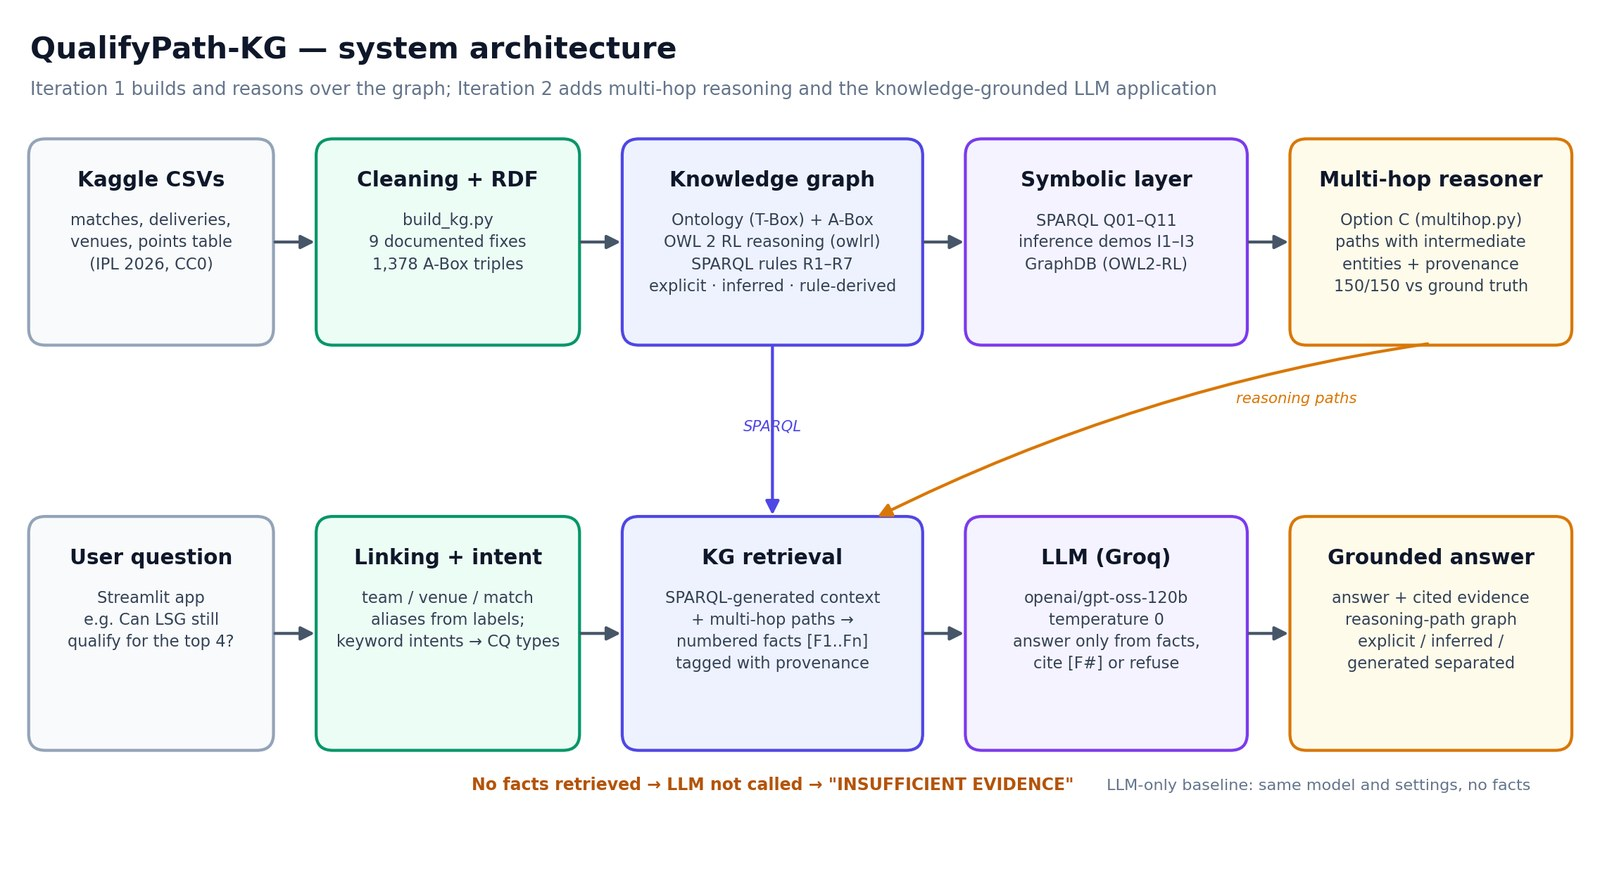
\includegraphics[width=\linewidth]{figures/architecture.jpg}
\caption{End-to-end architecture. Top: Iteration~1 knowledge graph and symbolic layer, plus the Iteration~2
multi-hop reasoner. Bottom: the question-answering pipeline.}
\label{fig:architecture}
\end{figure}

\section{Dataset and data preparation}

\subsection{Source}
We use the \emph{IPL 2026 -- Complete Dataset} by Data Knight on Kaggle \citep{kaggleipl2026} (CC0 public
domain; compiled from ESPNcricinfo, the IPL website and Google). The untouched archive is kept in
\texttt{Dataset/ipl-2026-complete-dataset.zip}.

\begin{table}[H]\centering\small
\begin{tabular}{p{4.2cm}p{3.6cm}p{7.2cm}}
\toprule
\textbf{File} & \textbf{Rows} & \textbf{Used for} \\ \midrule
\texttt{matches.csv} & 39 (matches 1--39) & results, scores, wickets, balls left $\rightarrow$ completed matches \\
\texttt{deliveries.csv} & 17{,}477 balls, all 74 matches & batting order, legal balls, teams/date/venue of matches 40--70 $\rightarrow$ fixtures \\
\texttt{venues.csv} & 12 & city and home team of each ground \\
\texttt{points\_table.csv} & 10 teams after match 39 & validation only (official table) \\
squads and player statistics & --- & not used: players are outside the qualification model \\
\bottomrule
\end{tabular}
\caption{Source files and how they are used.}
\end{table}

\subsection{Cleaning and transformation}
All cleaning is performed by \texttt{RDF\_Knowledge\_Graph/build\_kg.py}, which writes the cleaned match table
(\texttt{Dataset/processed/league\_matches\_clean.csv}) and the RDF instance data.

\begin{table}[H]\centering\small
\begin{tabular}{p{5.2cm}p{9.9cm}}
\toprule
\textbf{Problem found} & \textbf{Resolution} \\ \midrule
Ball-by-ball runs differ from the scorecard in 23 innings (1--3 runs) & Runs and wickets taken from \texttt{matches.csv}; ball-by-ball data only for batting order, legal balls and fixtures \\
Match 32 winner recorded as LSG; RR actually won by 40 runs & Winner derived from the scores; \texttt{match\_winner} trusted only for super-over ties \\
Match 13 rain-shortened to 11 overs a side & Detected automatically; stored as \texttt{qp:oversPerSide 11} for the NRR rule \\
Overs such as 19.4 cannot be used in arithmetic & Balls faced stored instead (19.4 overs $=$ 118 balls) \\
All-out innings count as the full quota for NRR & \texttt{qp:allOut} flag; rule R2 uses the quota \\
Venue names spelled up to three ways; two venues missing & Keyword matching to one canonical venue per ground; Raipur and Dharamshala added (13 venues) \\
Team abbreviations vs.\ full names & One team resource with \texttt{qp:shortName} and \texttt{rdfs:label} \\
Two date formats & Converted to \texttt{xsd:date} \\
Abandoned match 12 and super-over balls & Match 12 is a \texttt{qp:NoResultMatch} with no innings; super-over innings ignored \\
\bottomrule
\end{tabular}
\caption{Data-quality problems and how they were resolved.}
\end{table}

\subsection{Validation}
After cleaning, the standings derived by our rules match the official points table after match~39 for all
ten teams on played, won, lost, no-result and points, and on NRR to three decimals for nine teams. The tenth,
KKR, is $-0.751$ in our graph and $+0.751$ in the file; with two wins and five losses a positive NRR is
implausible and the magnitude matches exactly, so we treat it as a dropped minus sign in the source.

\textbf{Iteration 2 correction.} Iteration~1 assumed NRR as the only tie-break. Researching the IPL playing
conditions showed that clause 16.10.2 ranks teams level on points first by \emph{most wins} and then by
\emph{NRR} \citep{crictracker2024tiebreak}. The ontology instance data and rule R7 now encode both criteria;
the positions after match~39 are unchanged because every pair level on points is also level on wins.

\section{Competency questions}
Fifteen competency questions (CQs) drove the ontology design. Tags: \textbf{MH} multi-hop, \textbf{INF} needs
inference, \textbf{AGG} aggregation/filtering, \textbf{LLM} hard for an LLM without the graph. Team~X is RR
(Rajasthan Royals) and Team~Z is KKR (Kolkata Knight Riders).

{\small
\begin{longtable}{p{1.0cm}p{12.1cm}p{2.0cm}}
\toprule \textbf{CQ} & \textbf{Question} & \textbf{Tags} \\ \midrule \endfirsthead
\toprule \textbf{CQ} & \textbf{Question} & \textbf{Tags} \\ \midrule \endhead
CQ1 & What is each team's points total, and how many matches has it played, won, lost and had with no result? & AGG \\
CQ2 & Which teams hold the qualifying places once points and the season's tie-break order are applied? & AGG, INF, LLM \\
CQ3 & What is RR's net run rate (runs per over scored minus runs per over conceded; an all-out innings counts as its full quota)? & AGG, LLM \\
CQ4 & Which remaining fixtures does RR still have to play, against whom, when and where? & MH \\
CQ5 & What is the highest points total RR can still reach if it wins all its remaining matches? & MH, AGG \\
CQ6 & Which teams are mathematically eliminated (their highest reachable total is below the points of at least as many teams as there are qualifying places)? & INF, AGG, LLM \\
CQ7 & Which teams have already qualified, because too few other teams can still reach their current total? & INF, LLM \\
CQ8 & Which of RR's remaining opponents are direct rivals still in contention for the same places? & MH, INF \\
CQ9 & Which remaining matches are between two teams that are both still in contention? & MH, INF \\
CQ10 & If KKR loses its last match, which teams finish above it on points, and which are level so that the tie-break decides? & MH, AGG, LLM \\
CQ11 & Which teams has RR beaten this season, and at which venues? & MH, INF \\
CQ12 & Which matches ended with no result, and how many points did each affected team receive? & INF, AGG \\
CQ13 & At which venues has RR played this season, and in which cities are they? & MH, INF \\
CQ14 & Which teams have won at least half of their decided matches at their home venue? & MH, AGG \\
CQ15 & Which qualification rules apply (points per result, qualifying places, tie-break order)? & LLM \\
\bottomrule
\caption{The fifteen competency questions.}\label{tab:cqs}
\end{longtable}}

\begin{table}[H]\centering\small
\begin{tabular}{lccl}
\toprule
\textbf{Category} & \textbf{Required} & \textbf{Have} & \textbf{CQs} \\ \midrule
Total & 12--15 & 15 & CQ1--CQ15 \\
Multi-hop & $\geq 4$ & 8 & CQ4, 5, 8, 9, 10, 11, 13, 14 \\
Inference & $\geq 2$ & 8 & CQ2, 6, 7, 8, 9, 11, 12, 13 \\
Aggregation / filtering & $\geq 2$ & 8 & CQ1, 2, 3, 5, 6, 10, 12, 14 \\
Hard for an LLM alone & $\geq 2$ & 6 & CQ2, 3, 6, 7, 10, 15 \\
\bottomrule
\end{tabular}
\caption{Requirement coverage of the competency questions.}
\end{table}

\subsection{CQ-to-KG mapping}
Codes O1--O5 are the OWL/RDFS constructs and R1--R7 the SPARQL rules described in Sections~\ref{sec:ontology}
and~\ref{sec:sparql}.

{\scriptsize
\begin{longtable}{p{0.8cm}p{3.3cm}p{3.4cm}p{2.4cm}p{4.4cm}}
\toprule \textbf{CQ} & \textbf{Classes} & \textbf{Properties} & \textbf{Rule / inference} & \textbf{Graph path} \\ \midrule \endfirsthead
\toprule \textbf{CQ} & \textbf{Classes} & \textbf{Properties} & \textbf{Rule / inference} & \textbf{Graph path} \\ \midrule \endhead
CQ1 & Team, CompletedMatch, DecidedMatch, NoResultMatch, Season, PointsRule & participatesIn, hasWinner, hasLoser, inSeason, pointsForWin, pointsForNoResult & O3, O4 classify matches; R1 points & Team $\rightarrow$ participatesIn $\rightarrow$ CompletedMatch $\rightarrow$ inSeason $\rightarrow$ Season $\rightarrow$ hasPointsRule \\
CQ2 & StandingEntry, Season, QualificationRule, TieBreakCriterion & points, won, netRunRate, qualifyingPlaces, hasTieBreak, tieBreakRank & R1, R2, R7 & StandingEntry $\rightarrow$ standingIn $\rightarrow$ Season $\rightarrow$ hasTieBreak (ordered by rank) \\
CQ3 & Team, Innings, CompletedMatch & battingTeam, bowlingTeam, runs, ballsFaced, allOut, oversPerSide & R2 net run rate & Team $\leftarrow$ battingTeam/bowlingTeam $\leftarrow$ Innings $\leftarrow$ hasInnings $\leftarrow$ Match \\
CQ4 & Team, ScheduledMatch, Venue, City & participatesIn, hasParticipant, matchDate, scheduledAt, locatedIn & ScheduledMatch disjoint with CompletedMatch & RR $\rightarrow$ participatesIn $\rightarrow$ ScheduledMatch $\rightarrow$ hasParticipant $\rightarrow$ opponent; $\rightarrow$ scheduledAt $\rightarrow$ Venue $\rightarrow$ City \\
CQ5 & Team, ScheduledMatch, StandingEntry, PointsRule & participatesIn, points, maxReachablePoints & R3 reachable points & Team $\rightarrow$ participatesIn $\rightarrow$ ScheduledMatch (count) + PointsRule \\
CQ6 & StandingEntry, EliminatedStanding, QualificationRule & points, maxReachablePoints, qualifyingPlaces & R3 $\rightarrow$ R4 & every StandingEntry compared with all others in the season \\
CQ7 & StandingEntry, QualifiedStanding & points, maxReachablePoints, qualifyingPlaces & R3 $\rightarrow$ R5 & as CQ6 \\
CQ8 & Team, ScheduledMatch, InContentionStanding & participatesIn, hasParticipant, standingOf & R4, R5 $\rightarrow$ R6 & RR $\rightarrow$ ScheduledMatch $\rightarrow$ opponent $\leftarrow$ standingOf $\leftarrow$ InContentionStanding \\
CQ9 & ScheduledMatch, InContentionStanding & hasParticipant, standingOf & R6 & ScheduledMatch $\rightarrow$ two teams, each $\leftarrow$ InContentionStanding \\
CQ10 & Team, ScheduledMatch, StandingEntry, TieBreakCriterion & participatesIn, matchDate, points, maxReachablePoints & what-if scenario over R1--R3 & KKR $\rightarrow$ last ScheduledMatch (max date) $\rightarrow$ opponent credited with the win \\
CQ11 & Team, DecidedMatch, Venue & hasWinner, hasLoser, playedAt & O1, O2, O3 & RR $\leftarrow$ hasWinner $\leftarrow$ DecidedMatch $\rightarrow$ hasLoser $\rightarrow$ team; $\rightarrow$ playedAt $\rightarrow$ Venue \\
CQ12 & NoResultMatch, CompletedMatch, PointsRule & hasParticipant, pointsForNoResult & O4; R1 & NoResultMatch $\rightarrow$ hasParticipant $\rightarrow$ Team \\
CQ13 & Team, Venue, City & playedAtVenue (inferred), locatedIn & O5 property chain & Team $\rightarrow$ playedAtVenue $\rightarrow$ Venue $\rightarrow$ City \\
CQ14 & Team, Venue, DecidedMatch & homeVenue, playedAt, hasWinner & GROUP BY + HAVING & Team $\rightarrow$ homeVenue $\rightarrow$ Venue $\leftarrow$ playedAt $\leftarrow$ Match \\
CQ15 & Season, Tournament, PointsRule, QualificationRule, TieBreakCriterion & hasPointsRule, hasQualificationRule, hasTieBreak, tieBreakRank & rules stored as data & Season $\rightarrow$ hasTieBreak, ordered by tieBreakRank \\
\bottomrule
\caption{CQ-to-KG mapping.}\label{tab:mapping}
\end{longtable}}

\section{Ontology and knowledge graph design}\label{sec:ontology}

\subsection{T-Box: classes, properties and constructs}
The schema (\texttt{Ontology/qualifypath.ttl}, \statTbox{} triples) defines \statClasses{} classes,
\statObjProps{} object properties and \statDataProps{} datatype properties in the namespace
\texttt{qp:~<http://example.org/qualifypath/ontology\#>}. The match hierarchy separates what has happened from
what is still to come: \texttt{CompletedMatch} (with subclasses \texttt{DecidedMatch} and
\texttt{NoResultMatch}) is disjoint with \texttt{ScheduledMatch}. Tournament rules (\texttt{PointsRule},
\texttt{QualificationRule}, \texttt{TieBreakCriterion}) are \emph{data} attached to a season, so a different
tournament only needs different rule instances. Standings live in \texttt{StandingEntry} resources whose status
subclasses are filled by rules, never loaded (\figref{fig:ontology_schema.jpg}).

\begin{figure}[H]\centering
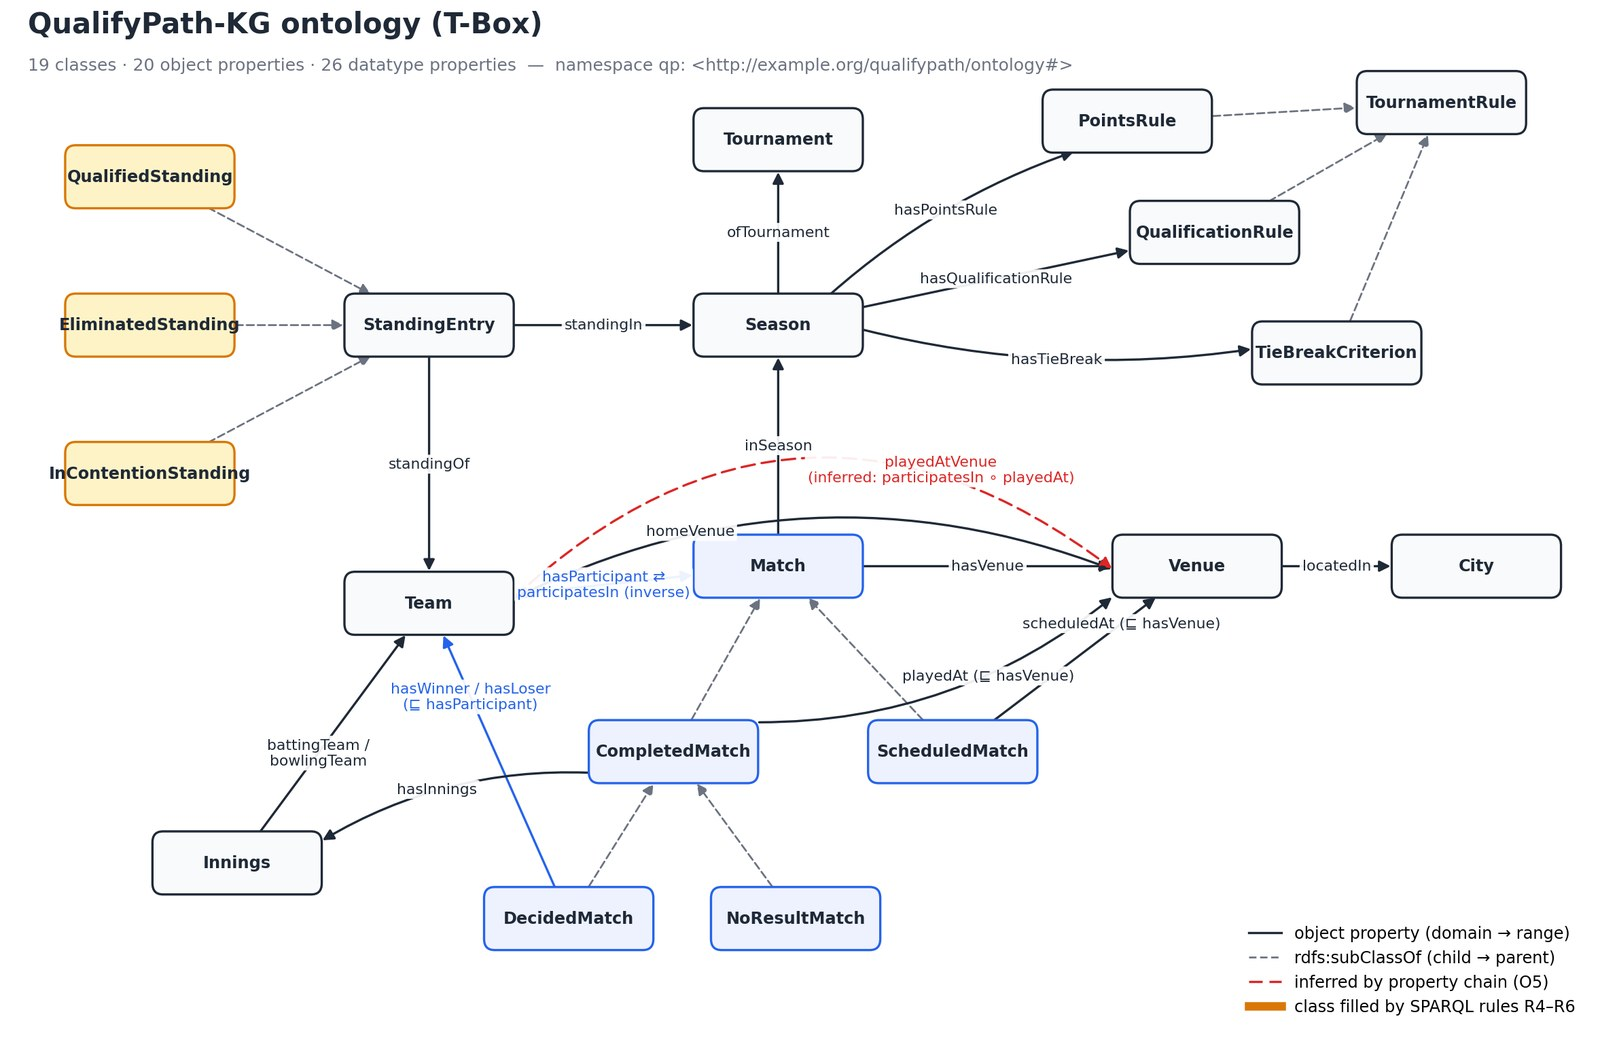
\includegraphics[width=\linewidth]{figures/ontology_schema.jpg}
\caption{Ontology (T-Box): classes, subclass links and object properties (domain $\rightarrow$ range). The red
dashed edge is inferred by a property chain; amber classes are filled by SPARQL rules R4--R6.}
\label{fig:ontology_schema.jpg}
\end{figure}

\begin{table}[H]\centering\small
\begin{tabular}{p{0.7cm}p{6.6cm}p{7.6cm}}
\toprule
\textbf{Code} & \textbf{Construct} & \textbf{What the reasoner infers} \\ \midrule
O1 & \texttt{hasWinner}, \texttt{hasLoser} \texttt{rdfs:subPropertyOf} \texttt{hasParticipant} & the winner and loser of a match are its participants \\
O2 & \texttt{participatesIn} \texttt{owl:inverseOf} \texttt{hasParticipant} & Team $\rightarrow$ participatesIn $\rightarrow$ Match without storing it twice \\
O3 & \texttt{hasWinner} \texttt{rdfs:domain} \texttt{DecidedMatch} & a match with a winner is a DecidedMatch \\
O4 & \texttt{DecidedMatch}, \texttt{NoResultMatch} \texttt{rdfs:subClassOf} \texttt{CompletedMatch} & decided and abandoned matches count as completed \\
O5 & \texttt{playedAtVenue} \texttt{owl:propertyChainAxiom} (\texttt{participatesIn} \texttt{playedAt}) & Team $\rightarrow$ playedAtVenue $\rightarrow$ Venue \\
\bottomrule
\end{tabular}
\caption{Reasoning-enabling constructs. Constraints (consistency checks): CompletedMatch $\sqcap$ ScheduledMatch
$=\emptyset$, a Match has exactly two participants, a DecidedMatch exactly one winner, status classes are
disjoint.}
\end{table}

OWL~2~RL \citep{w3c2012owl2profiles} was chosen because it is the rule-based profile that both
\texttt{owlrl} (Python) and GraphDB's OWL2-RL ruleset implement, and it supports every construct above,
including property chains. Arithmetic (points, NRR, positions) is outside OWL, so it is done by SPARQL Update
rules (Section~\ref{sec:sparql}).

\textbf{Improvements in Iteration 2.} \texttt{playedAt} is now restricted to completed matches and a new
\texttt{scheduledAt} (both sub-properties of \texttt{hasVenue}) covers fixtures, after the reasoner showed that
the venue chain also counted future fixtures; \texttt{oversPerSide} handles rain-shortened matches; and the
tie-break order follows IPL clause 16.10.2.

\subsection{A-Box and URI design}
The instance data (\texttt{RDF\_Knowledge\_Graph/ipl2026\_abox.ttl}) has \statAbox{} triples; with the
ontology the graph holds \statExplicit{} explicit triples --- well above the 500 required --- and grows to
\statFull{} after OWL~2~RL reasoning (\statInferred{} inferred) and the rules (\statRule{} rule-derived).
Decided matches are stored only as \texttt{qp:Match} with \texttt{hasWinner}/\texttt{hasLoser}; that they are
completed, decided and who participated is left to the reasoner.

\begin{table}[H]\centering\small
\begin{tabular}{p{2.3cm}p{6.4cm}p{6.2cm}}
\toprule
\textbf{Resource} & \textbf{Pattern} (\texttt{\ldots/resource/}) & \textbf{Example} \\ \midrule
Ontology term & \texttt{\ldots/ontology\#<Term>} & \texttt{qp:DecidedMatch} \\
Team & \texttt{team/<official abbreviation>} & \texttt{team:RR} \\
Venue / City & \texttt{venue/<slug>}, \texttt{city/<slug>} & \texttt{venue:eden-gardens} \\
Season & \texttt{season/<tournament>-<year>} & \texttt{season:IPL-2026} \\
Match & \texttt{match/<season>-M<number>} & \texttt{match:IPL-2026-M32} \\
Innings & \texttt{innings/<match>-<n>} & \texttt{innings:IPL-2026-M32-1} \\
Rule & \texttt{rule/<season>-<rule>} & \texttt{rule:IPL-2026-tiebreak-1} \\
Standing & \texttt{standing/<season>-<team>} (rule-created) & \texttt{standing:IPL-2026-RR} \\
\bottomrule
\end{tabular}
\caption{URI design: readable, stable identifiers from official codes; season-scoped where a resource belongs to
one season; names kept in \texttt{rdfs:label} so spelling variants never create duplicates.}
\end{table}

\subsection{Knowledge graph visualisation}
\begin{figure}[H]\centering
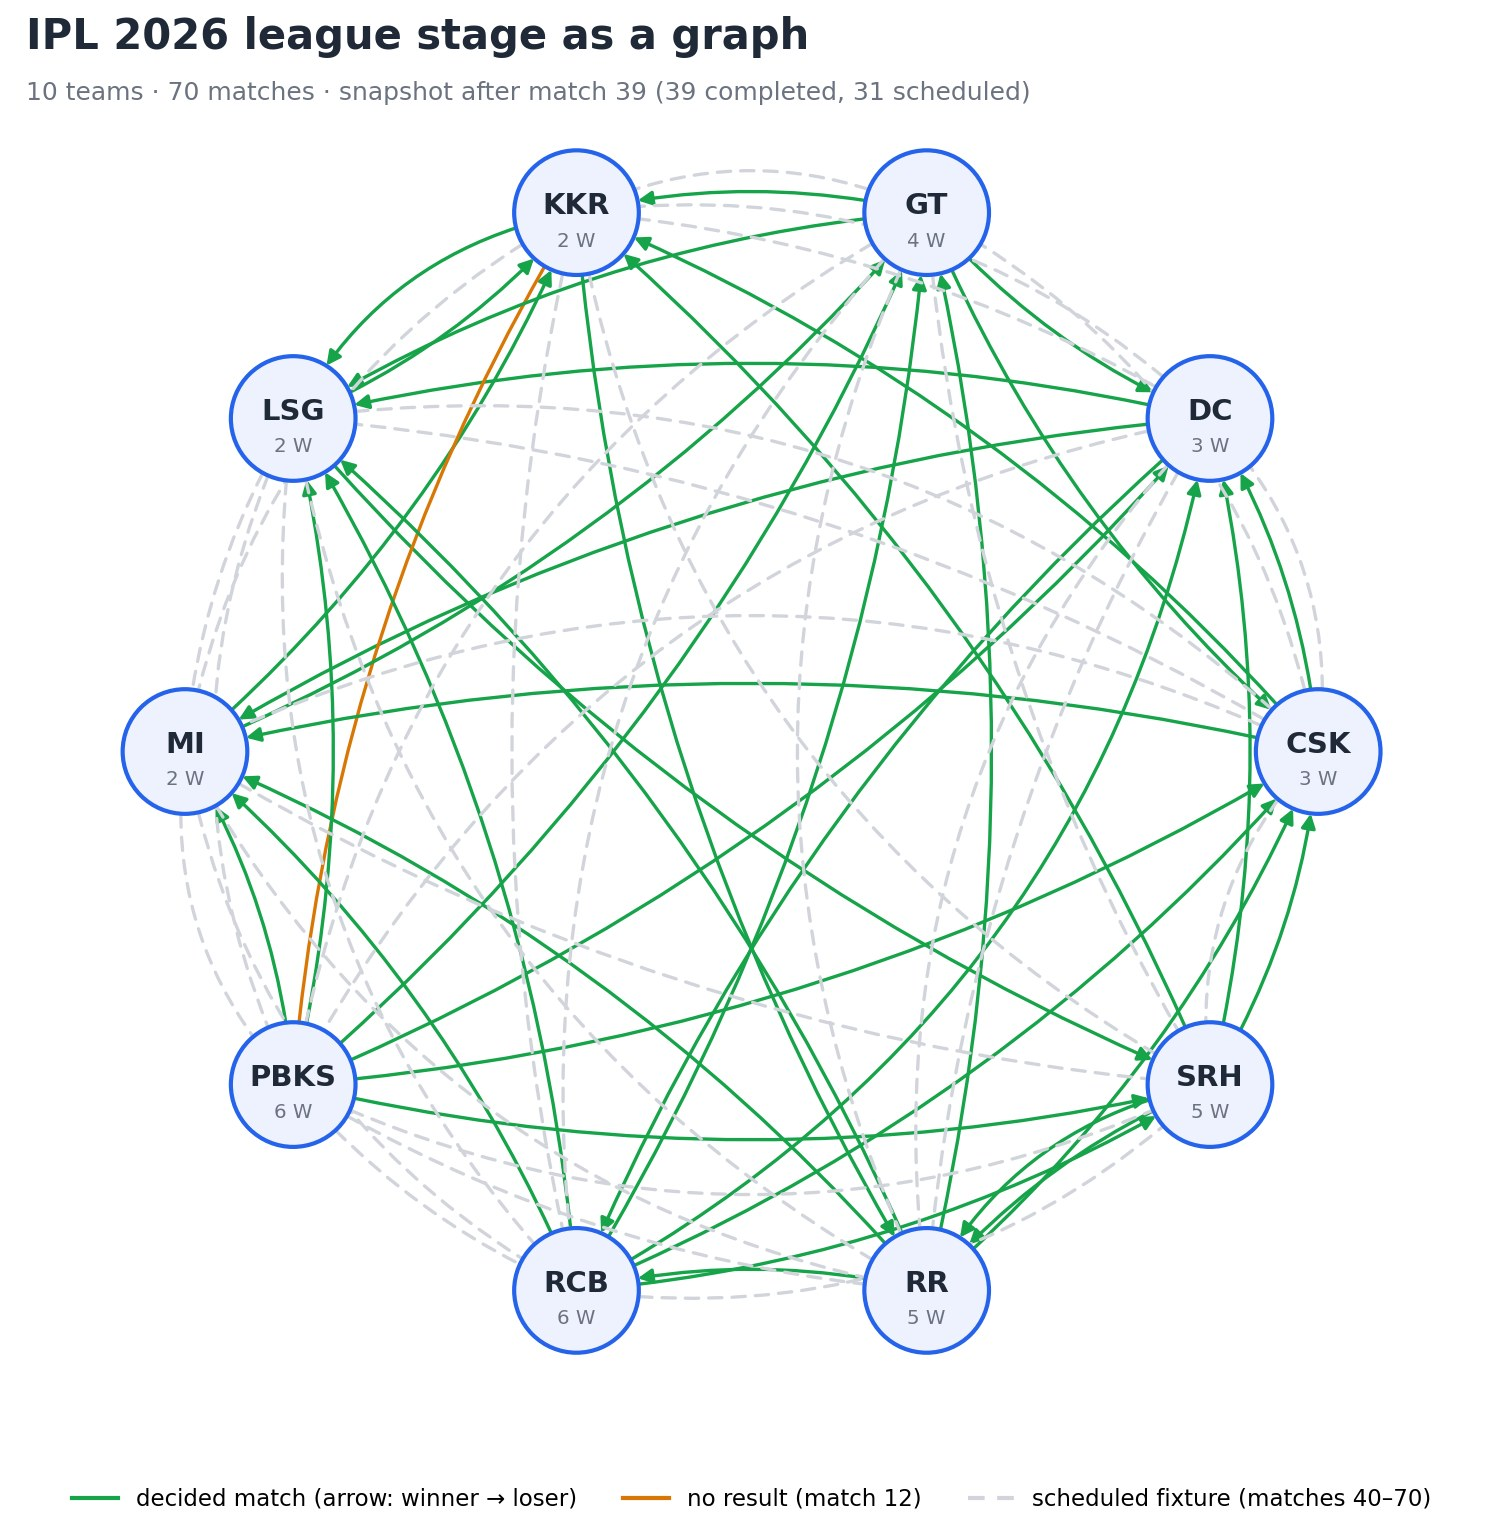
\includegraphics[width=0.78\linewidth]{figures/season_graph.jpg}
\caption{The league stage as a graph: ten teams, each of the 70 matches an edge (winner $\rightarrow$ loser,
no result, or scheduled).}
\end{figure}
\shot[0.92\linewidth]{rr_neighbourhood.jpg}{Instance level: RR, its 14 matches, opponents and venue cities.}
\shot[0.9\linewidth]{graphdb_class_hierarchy.jpg}{GraphDB class hierarchy of the loaded repository
(\texttt{qualifypath-ipl2026}, OWL2-RL ruleset).}
\shot[0.9\linewidth]{graphdb_visual_graph_match03.jpg}{GraphDB visual graph of match~3: the types
\emph{Completed match} and \emph{Decided match} are inferred, not stored.}
\shot[0.9\linewidth]{graphdb_visual_graph_RR.jpg}{GraphDB visual graph of RR: its matches, the venues it has
played at (inferred) and its standing entry.}

\section{SPARQL queries and symbolic reasoning}\label{sec:sparql}

\subsection{Rules R1--R7 as SPARQL Update}
Points, NRR and qualification need arithmetic and counting, which OWL cannot express, so they are implemented
as SPARQL~1.1 Update rules \citep{w3c2013sparqlupdate} that materialise one \texttt{qp:StandingEntry} per team.
They run after OWL~2~RL reasoning, because they rely on inferred facts such as \texttt{CompletedMatch} and
\texttt{participatesIn}.

\begin{table}[H]\centering\small
\begin{tabular}{p{1.3cm}p{13.6cm}}
\toprule
\textbf{Rule} & \textbf{Definition} \\ \midrule
R1 & points $=$ won $\times$ pointsForWin $+$ lost $\times$ pointsForLoss $+$ noResult $\times$ pointsForNoResult \\
R2 & NRR $=$ runs scored / overs faced $-$ runs conceded / overs bowled (overs $=$ balls/6; all out $=$ full quota; shortened matches use \texttt{oversPerSide}) \\
R3 & maxReachablePoints $=$ points $+$ remaining fixtures $\times$ pointsForWin \\
R4 & EliminatedStanding if at least \emph{qualifyingPlaces} other teams already have more points than this team can reach \\
R5 & QualifiedStanding if fewer than \emph{qualifyingPlaces} other teams can still reach this team's points \\
R6 & InContentionStanding otherwise \\
R7 & position: more points, then more wins (tie-break 1), then higher NRR (tie-break 2) \\
\bottomrule
\end{tabular}
\caption{SPARQL Update rules (\texttt{SPARQL\_Queries/rules/}). R4 and R5 use points only, so they never
wrongly declare a team qualified or eliminated, but may keep a team ``in contention'' longer than the official
table.}
\end{table}

\lstinputlisting[language=SPARQL,caption={Rule R7 (position with the IPL tie-break order).}]{generated/queries/R7_position.ru}

The derived league table (\tabref{tab:standings}) is identical to the official IPL table after match~39.

\begin{table}[H]\centering
{\small
\begin{tabular}{rlrrl}
\toprule
\textbf{position} & \textbf{team} & \textbf{points} & \textbf{netRunRate} & \textbf{inQualifyingPlace} \\
\midrule
1 & PBKS & 13 & 1.333 & True \\
2 & RCB & 12 & 1.919 & True \\
3 & SRH & 10 & 0.815 & True \\
4 & RR & 10 & 0.602 & True \\
5 & GT & 8 & -0.475 & False \\
6 & CSK & 6 & -0.121 & False \\
7 & DC & 6 & -1.06 & False \\
8 & KKR & 5 & -0.751 & False \\
9 & MI & 4 & -0.736 & False \\
10 & LSG & 4 & -1.106 & False \\
\bottomrule
\end{tabular}}

\caption{League positions derived by rules R1--R7 (query Q04).}\label{tab:standings}
\end{table}

\subsection{The eleven SPARQL queries}
\begin{table}[H]\centering\small
\begin{tabular}{p{4.2cm}p{10.6cm}}
\toprule
\textbf{Required feature} & \textbf{Queries} \\ \midrule
Basic graph pattern & Q01 \\
FILTER & Q05, Q06, Q09, Q11 \\
OPTIONAL / UNION & Q03 (OPTIONAL), Q09 (UNION and OPTIONAL) \\
Aggregation & Q02, Q03, Q10 (with HAVING) \\
Multi-hop traversal & Q05, Q07, Q11 \\
Property paths & Q01, Q04, Q05, Q07 (inverse path \texttt{\^{}qp:hasWinner}) \\
Inference-dependent & Q02, Q08 (and rule-derived classes in Q04, Q06, Q11) \\
\bottomrule
\end{tabular}
\caption{SPARQL feature coverage.}
\end{table}

Every query below was run on the graph after OWL~2~RL reasoning and the rules; the same results are returned by
GraphDB (\figref{fig:graphdb_sparql_Q05.jpg}, \figref{fig:graphdb_sparql_Q04.jpg}).

\subsubsection*{Q01 --- season rules (CQ15; basic graph pattern, property path)}
\lstinputlisting[language=SPARQL]{generated/queries/Q01_season_rules.rq}
\noindent\textit{Output (2 rows):}\par\smallskip
\resizebox{\ifdim\width>\linewidth\linewidth\else\width\fi}{!}{{\footnotesize
\begin{tabular}{llllllll}
\toprule
\textbf{season} & \textbf{pointsForWin} & \textbf{pointsForLoss} & \textbf{pointsForNoResult} & \textbf{oversQuota} & \textbf{qualifyingPlaces} & \textbf{tieBreakRank} & \textbf{tieBreak} \\
\midrule
IPL 2026 & 2 & 0 & 1 & 20 & 4 & 1 & Most wins \\
IPL 2026 & 2 & 0 & 1 & 20 & 4 & 2 & Net run rate \\
\bottomrule
\end{tabular}}}
\medskip
\subsubsection*{Q02 --- points table (CQ1; aggregation, inference-dependent)}
\lstinputlisting[language=SPARQL]{generated/queries/Q02_points_table.rq}
\noindent\textit{Output (10 rows):}\par\smallskip
\resizebox{\ifdim\width>\linewidth\linewidth\else\width\fi}{!}{{\footnotesize
\begin{tabular}{llllll}
\toprule
\textbf{team} & \textbf{played} & \textbf{won} & \textbf{lost} & \textbf{noResult} & \textbf{points} \\
\midrule
PBKS & 7 & 6 & 0 & 1 & 13 \\
RCB & 8 & 6 & 2 & 0 & 12 \\
RR & 8 & 5 & 3 & 0 & 10 \\
SRH & 8 & 5 & 3 & 0 & 10 \\
GT & 8 & 4 & 4 & 0 & 8 \\
CSK & 8 & 3 & 5 & 0 & 6 \\
DC & 8 & 3 & 5 & 0 & 6 \\
KKR & 8 & 2 & 5 & 1 & 5 \\
\multicolumn{6}{l}{\textit{\ldots{} 2 more rows}} \\
\bottomrule
\end{tabular}}}
\medskip
\subsubsection*{Q03 --- net run rate (CQ3; aggregation, OPTIONAL, VALUES)}
\lstinputlisting[language=SPARQL]{generated/queries/Q03_net_run_rate.rq}
\noindent\textit{Output (10 rows):}\par\smallskip
\resizebox{\ifdim\width>\linewidth\linewidth\else\width\fi}{!}{{\footnotesize
\begin{tabular}{llllll}
\toprule
\textbf{team} & \textbf{runsFor} & \textbf{ballsFaced} & \textbf{runsAgainst} & \textbf{ballsBowled} & \textbf{netRunRate} \\
\midrule
RCB & 1501 & 817 & 1437 & 947 & 1.919 \\
PBKS & 1315 & 672 & 1249 & 720 & 1.333 \\
SRH & 1683 & 951 & 1513 & 926 & 0.815 \\
RR & 1391 & 847 & 1380 & 895 & 0.602 \\
CSK & 1496 & 960 & 1397 & 885 & -0.121 \\
GT & 1389 & 930 & 1491 & 948 & -0.475 \\
MI & 1229 & 781 & 1279 & 754 & -0.736 \\
KKR & 1218 & 838 & 1315 & 833 & -0.751 \\
\multicolumn{6}{l}{\textit{\ldots{} 2 more rows}} \\
\bottomrule
\end{tabular}}}
\medskip
\subsubsection*{Q04 --- qualifying places (CQ2; property path, rule results)}
\lstinputlisting[language=SPARQL]{generated/queries/Q04_qualifying_places.rq}
\noindent\textit{Output (10 rows):}\par\smallskip
\resizebox{\ifdim\width>\linewidth\linewidth\else\width\fi}{!}{{\footnotesize
\begin{tabular}{lllll}
\toprule
\textbf{position} & \textbf{team} & \textbf{points} & \textbf{netRunRate} & \textbf{inQualifyingPlace} \\
\midrule
1 & PBKS & 13 & 1.333 & True \\
2 & RCB & 12 & 1.919 & True \\
3 & SRH & 10 & 0.815 & True \\
4 & RR & 10 & 0.602 & True \\
5 & GT & 8 & -0.475 & False \\
6 & CSK & 6 & -0.121 & False \\
7 & DC & 6 & -1.06 & False \\
8 & KKR & 5 & -0.751 & False \\
\multicolumn{5}{l}{\textit{\ldots{} 2 more rows}} \\
\bottomrule
\end{tabular}}}
\medskip
\subsubsection*{Q05 --- remaining fixtures (CQ4; multi-hop, FILTER, property path)}
\lstinputlisting[language=SPARQL]{generated/queries/Q05_remaining_fixtures.rq}
\noindent\textit{Output (6 rows):}\par\smallskip
\resizebox{\ifdim\width>\linewidth\linewidth\else\width\fi}{!}{{\footnotesize
\begin{tabular}{lllll}
\toprule
\textbf{matchNumber} & \textbf{date} & \textbf{opponent} & \textbf{venue} & \textbf{city} \\
\midrule
40 & 2026-04-28 & PBKS & Maharaja Yadavindra Singh International Cricket Stadium & Mullanpur \\
43 & 2026-05-01 & DC & Sawai Mansingh Stadium & Jaipur \\
52 & 2026-05-09 & GT & Sawai Mansingh Stadium & Jaipur \\
62 & 2026-05-17 & DC & Arun Jaitley Stadium & New Delhi \\
64 & 2026-05-19 & LSG & Sawai Mansingh Stadium & Jaipur \\
69 & 2026-05-24 & MI & Wankhede Stadium & Mumbai \\
\bottomrule
\end{tabular}}}
\medskip
\subsubsection*{Q06 --- qualification status (CQ5--CQ7; rule-inferred classes, FILTER)}
\lstinputlisting[language=SPARQL]{generated/queries/Q06_qualification_status.rq}
\noindent\textit{Output (10 rows):}\par\smallskip
\resizebox{\ifdim\width>\linewidth\linewidth\else\width\fi}{!}{{\footnotesize
\begin{tabular}{lllll}
\toprule
\textbf{team} & \textbf{points} & \textbf{remainingFixtures} & \textbf{maxReachablePoints} & \textbf{status} \\
\midrule
PBKS & 13 & 7 & 27 & In-contention standing \\
RCB & 12 & 6 & 24 & In-contention standing \\
SRH & 10 & 6 & 22 & In-contention standing \\
RR & 10 & 6 & 22 & In-contention standing \\
GT & 8 & 6 & 20 & In-contention standing \\
CSK & 6 & 6 & 18 & In-contention standing \\
DC & 6 & 6 & 18 & In-contention standing \\
KKR & 5 & 6 & 17 & In-contention standing \\
\multicolumn{5}{l}{\textit{\ldots{} 2 more rows}} \\
\bottomrule
\end{tabular}}}
\medskip
\subsubsection*{Q07 --- teams beaten (CQ11; multi-hop, inverse property path)}
\lstinputlisting[language=SPARQL]{generated/queries/Q07_teams_beaten.rq}
\noindent\textit{Output (5 rows):}\par\smallskip
\resizebox{\ifdim\width>\linewidth\linewidth\else\width\fi}{!}{{\footnotesize
\begin{tabular}{lllll}
\toprule
\textbf{matchNumber} & \textbf{date} & \textbf{beaten} & \textbf{venue} & \textbf{city} \\
\midrule
3 & 2026-03-30 & CSK & Barsapara Cricket Stadium & Guwahati \\
9 & 2026-04-04 & GT & Narendra Modi Stadium & Ahmedabad \\
13 & 2026-04-07 & MI & Barsapara Cricket Stadium & Guwahati \\
16 & 2026-04-10 & RCB & Barsapara Cricket Stadium & Guwahati \\
32 & 2026-04-22 & LSG & Bharat Ratna Shri Atal Bihari Vajpayee Ekana Cricket Stadium & Lucknow \\
\bottomrule
\end{tabular}}}
\medskip
\subsubsection*{Q08 --- venues played (CQ13; inference-dependent (property chain))}
\lstinputlisting[language=SPARQL]{generated/queries/Q08_venues_played.rq}
\noindent\textit{Output (6 rows):}\par\smallskip
\resizebox{\ifdim\width>\linewidth\linewidth\else\width\fi}{!}{{\footnotesize
\begin{tabular}{ll}
\toprule
\textbf{venue} & \textbf{city} \\
\midrule
Narendra Modi Stadium & Ahmedabad \\
Barsapara Cricket Stadium & Guwahati \\
Rajiv Gandhi International Stadium & Hyderabad \\
Sawai Mansingh Stadium & Jaipur \\
Eden Gardens & Kolkata \\
Bharat Ratna Shri Atal Bihari Vajpayee Ekana Cricket Stadium & Lucknow \\
\bottomrule
\end{tabular}}}
\medskip
\subsubsection*{Q09 --- team results (CQ12; UNION, OPTIONAL, FILTER)}
\lstinputlisting[language=SPARQL]{generated/queries/Q09_team_results.rq}
\noindent\textit{Output (8 rows):}\par\smallskip
\resizebox{\ifdim\width>\linewidth\linewidth\else\width\fi}{!}{{\footnotesize
\begin{tabular}{llllll}
\toprule
\textbf{matchNumber} & \textbf{date} & \textbf{opponent} & \textbf{result} & \textbf{points} & \textbf{shortenedTo} \\
\midrule
2 & 2026-03-29 & MI & Lost & 0 &  \\
6 & 2026-04-02 & SRH & Lost & 0 &  \\
12 & 2026-04-06 & PBKS & No result & 1 &  \\
15 & 2026-04-09 & LSG & Lost & 0 &  \\
22 & 2026-04-14 & CSK & Lost & 0 &  \\
25 & 2026-04-17 & GT & Lost & 0 &  \\
28 & 2026-04-19 & RR & Won & 2 &  \\
38 & 2026-04-26 & LSG & Won & 2 &  \\
\bottomrule
\end{tabular}}}
\medskip
\subsubsection*{Q10 --- home win ratio (CQ14; aggregation with HAVING)}
\lstinputlisting[language=SPARQL]{generated/queries/Q10_home_win_ratio.rq}
\noindent\textit{Output (6 rows):}\par\smallskip
\resizebox{\ifdim\width>\linewidth\linewidth\else\width\fi}{!}{{\footnotesize
\begin{tabular}{llll}
\toprule
\textbf{team} & \textbf{homeMatches} & \textbf{homeWins} & \textbf{winPercent} \\
\midrule
PBKS & 3 & 3 & 100 \\
RCB & 5 & 4 & 80 \\
RR & 4 & 3 & 75 \\
SRH & 4 & 3 & 75 \\
CSK & 3 & 2 & 67 \\
GT & 4 & 2 & 50 \\
\bottomrule
\end{tabular}}}
\medskip
\subsubsection*{Q11 --- rival fixtures (CQ8--CQ9; multi-hop, rule-inferred class)}
\lstinputlisting[language=SPARQL]{generated/queries/Q11_rival_fixtures.rq}
\noindent\textit{Output (6 rows):}\par\smallskip
\resizebox{\ifdim\width>\linewidth\linewidth\else\width\fi}{!}{{\footnotesize
\begin{tabular}{lllllll}
\toprule
\textbf{matchNumber} & \textbf{date} & \textbf{opponent} & \textbf{opponentPosition} & \textbf{opponentPoints} & \textbf{rrPoints} & \textbf{pointsGap} \\
\midrule
52 & 2026-05-09 & GT & 5 & 8 & 10 & 2 \\
40 & 2026-04-28 & PBKS & 1 & 13 & 10 & 3 \\
43 & 2026-05-01 & DC & 7 & 6 & 10 & 4 \\
62 & 2026-05-17 & DC & 7 & 6 & 10 & 4 \\
64 & 2026-05-19 & LSG & 10 & 4 & 10 & 6 \\
69 & 2026-05-24 & MI & 9 & 4 & 10 & 6 \\
\bottomrule
\end{tabular}}}
\medskip


\shot[0.95\linewidth]{graphdb_sparql_Q05.jpg}{Multi-hop query Q05 executed in GraphDB: RR's six remaining
fixtures with opponents, dates, venues and cities.}
\shot[0.95\linewidth]{graphdb_sparql_Q04.jpg}{Q04 in GraphDB: positions 1--10 match the official table.}

\subsection{Symbolic inference examples}
Each example follows the pattern \emph{explicit facts $\rightarrow$ rule or schema knowledge $\rightarrow$
inferred fact}, and is demonstrated by running the same query with inference switched off and on.

\paragraph{Example 1 --- the winner of a match took part in it (O1).}
Explicit: \texttt{match:IPL-2026-M01 qp:hasWinner team:RCB ; qp:hasLoser team:SRH}.
Rule: \texttt{hasWinner} and \texttt{hasLoser} are sub-properties of \texttt{hasParticipant}.
Inferred: \texttt{match:IPL-2026-M01 qp:hasParticipant team:RCB, team:SRH}. All 76 participation links of
decided matches are inferred this way.

\paragraph{Example 2 --- a match with a winner is a completed match (O3, O4).}
Explicit: \texttt{match:IPL-2026-M01 a qp:Match ; qp:hasWinner team:RCB}.
Rules: the domain of \texttt{hasWinner} is \texttt{DecidedMatch}, and \texttt{DecidedMatch} is a subclass of
\texttt{CompletedMatch}. Inferred: match~1 is a \texttt{DecidedMatch} and a \texttt{CompletedMatch}.
Season-wide, 0 completed matches are stored and 39 are inferred; the points table (Q02) depends on this.

\paragraph{Example 3 --- the venues a team has played at (O1, O2, O5).}
Explicit: \texttt{match:IPL-2026-M03 qp:hasWinner team:RR ; qp:playedAt venue:barsapara-cricket-stadium}.
Rules: sub-property (O1), inverse (O2) and the chain \texttt{playedAtVenue $\equiv$ participatesIn $\circ$ playedAt} (O5).
Inferred: \texttt{team:RR qp:participatesIn match:IPL-2026-M03} and
\texttt{team:RR qp:playedAtVenue venue:barsapara-cricket-stadium}. Season-wide, 0 team--venue links are stored
and 50 are inferred.

\begin{table}[H]\centering
{\footnotesize
\begin{tabular}{lrrp{8.2cm}}
\toprule
\textbf{Query} & \textbf{Off} & \textbf{On} & \textbf{Values with inference} \\
\midrule
I1\_winner\_is\_participant & 0 & 2 & RCB; SRH \\
I2\_match\_classified\_completed & 1 & 3 & qp:CompletedMatch; qp:DecidedMatch; qp:Match \\
I3\_team\_played\_at\_venue & 0 & 6 & Barsapara Cricket Stadium; Bharat Ratna Shri Atal Bihari Vajpayee Ekana Cricket Stadium; E... \\
season-wide (explicit) &  &  & CompletedMatch=0, DecidedMatch=0, team-venue pairs=0 \\
season-wide (inferred) &  &  & CompletedMatch=39, DecidedMatch=38, team-venue pairs=50 \\
\bottomrule
\end{tabular}}

\caption{Inference demonstrations I1--I3: rows returned with inference off and on.}
\end{table}

\begin{figure}[H]\centering
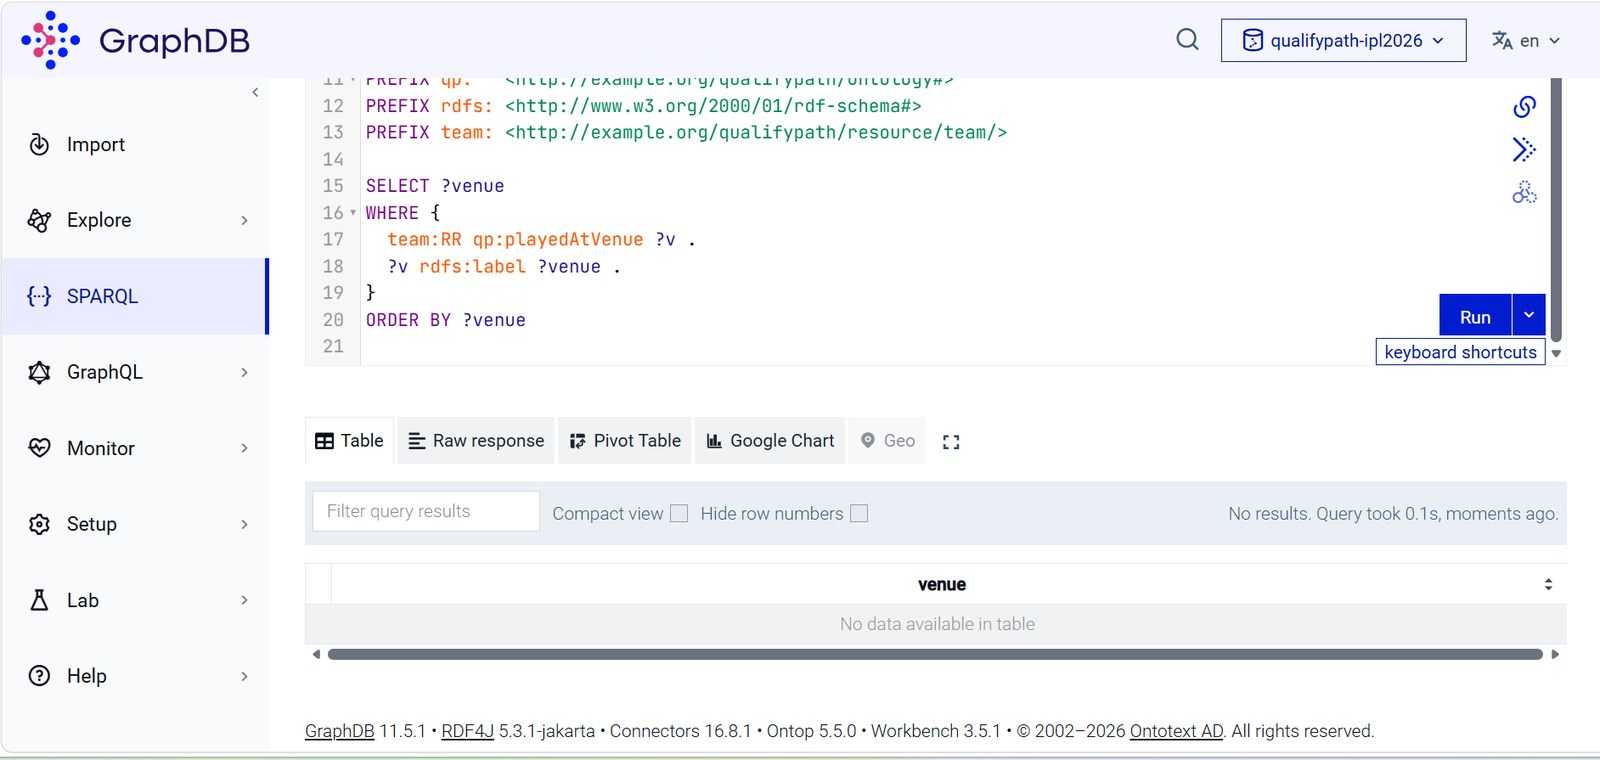
\includegraphics[width=0.49\linewidth]{figures/graphdb_inference_I3_off.jpg}\hfill
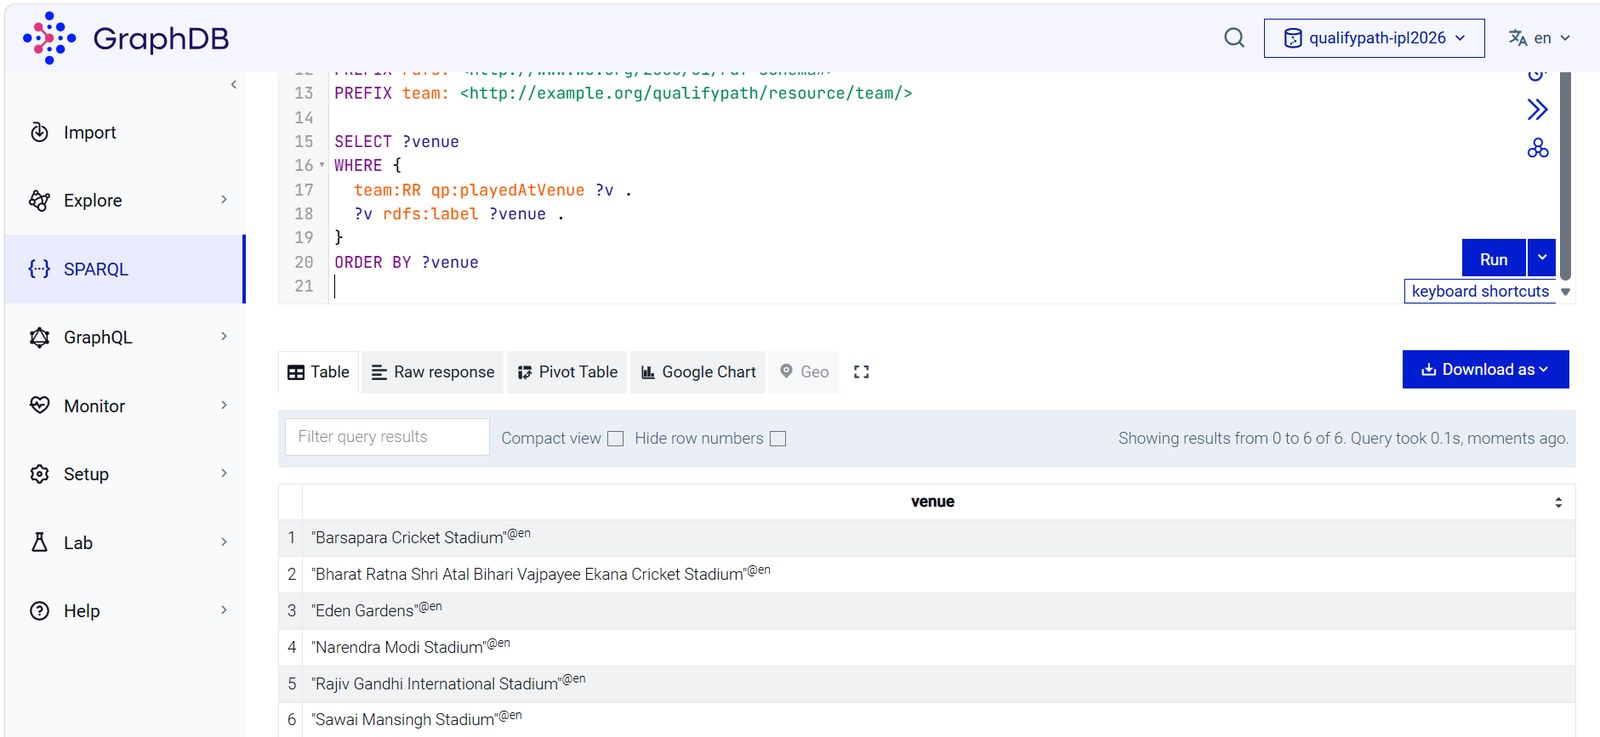
\includegraphics[width=0.49\linewidth]{figures/graphdb_inference_I3_on.jpg}
\caption{I3 in GraphDB with \emph{Include inferred data} off (left, no results) and on (right, six venues).}
\end{figure}
\begin{figure}[H]\centering
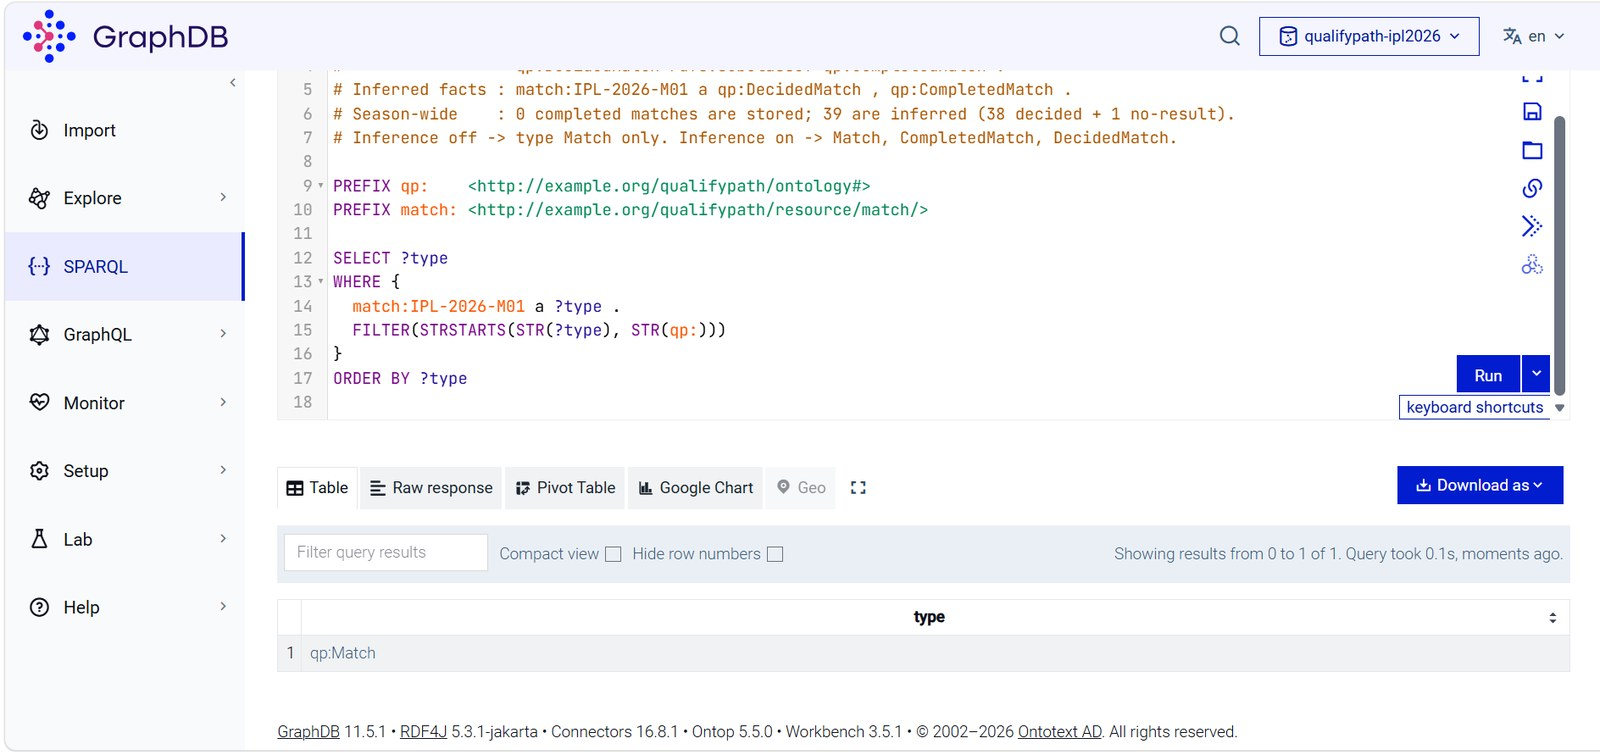
\includegraphics[width=0.49\linewidth]{figures/graphdb_inference_I2_off.jpg}\hfill
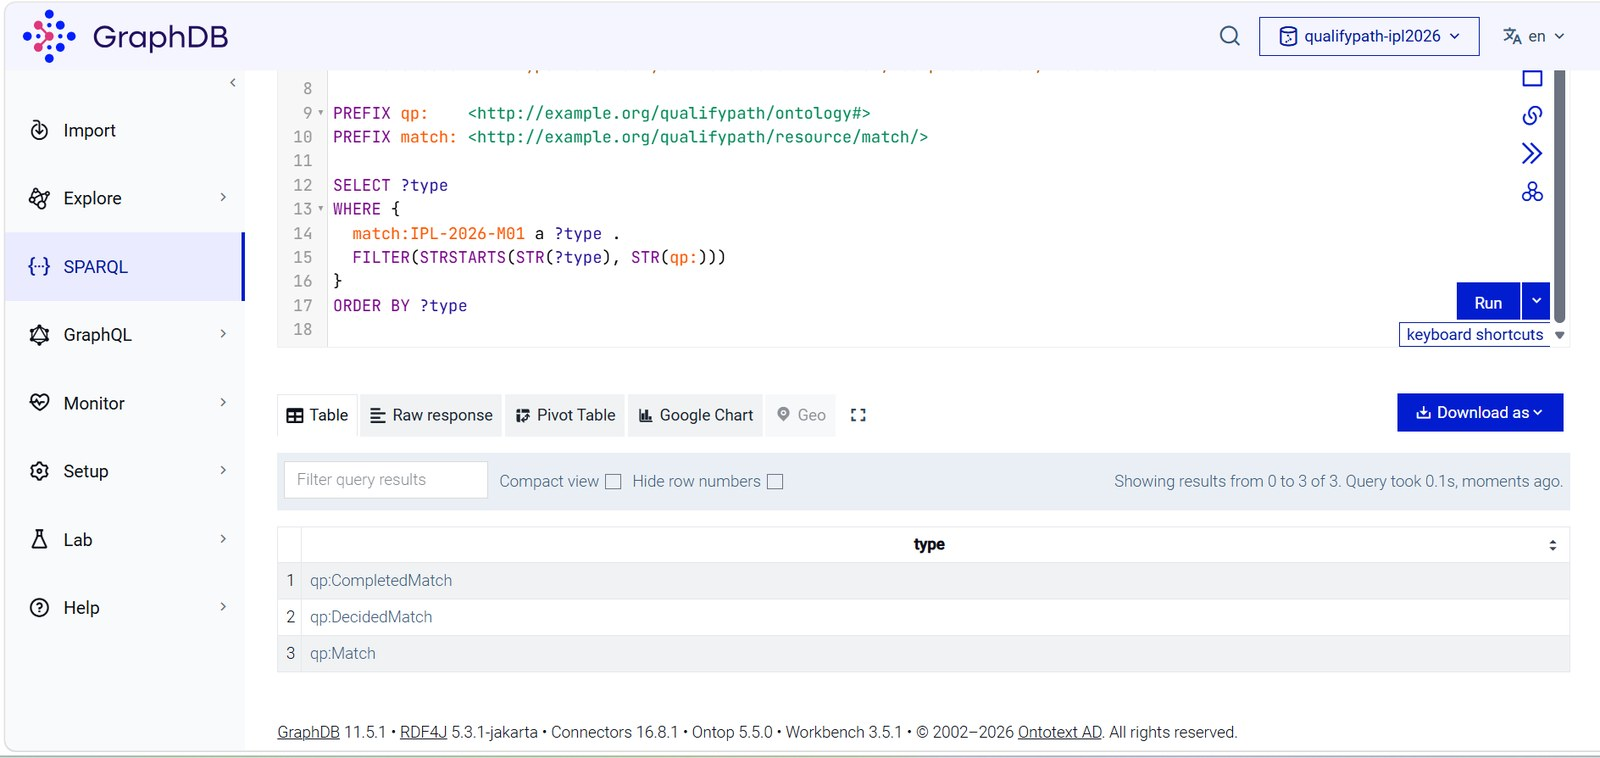
\includegraphics[width=0.49\linewidth]{figures/graphdb_inference_I2_on.jpg}
\caption{I2 in GraphDB: match~1 is only a \texttt{qp:Match} when inference is off, and also a
\texttt{CompletedMatch} and \texttt{DecidedMatch} when it is on.}
\end{figure}

\section{Modern KG reasoning: multi-hop reasoning (Option C)}\label{sec:multihop}

\subsection{Background and research}
Multi-hop reasoning answers a question by following several connected relationships, so the answer is the end
of a \emph{path} and the path itself is the explanation. Lao et al.\ \citep{lao2011pra} showed that sequences of
relations (relation paths) are informative features for inference in large knowledge bases; MINERVA
\citep{das2018minerva} learned to walk from a query entity to the answer, returning the walk as evidence; and
Think-on-Graph \citep{sun2024tog} lets an LLM explore graph paths step by step so that answers stay
traceable. Hogan et al.\ \citep{hogan2021knowledge} place these methods alongside deductive (rule-based)
reasoning and stress that graph paths make conclusions explainable.

\textbf{What we took from the literature.} From path-ranking work we took the idea that each question type is
a \emph{relation-path pattern} (for example \texttt{participatesIn} $\rightarrow$ \texttt{hasParticipant}
$\rightarrow$ \texttt{standingOf}$^{-1}$). From MINERVA and Think-on-Graph we took the principle that the
returned path, with every intermediate entity, is part of the answer. We did not train a learned walker:
our graph is small (about four thousand triples) and the answers must be exactly right, so deterministic graph
traversal over relation patterns is both sufficient and verifiable, while learned walkers are designed for
large, incomplete graphs.

\subsection{Method}
The reasoner (\texttt{qualifypath/multihop.py}) works on the graph after OWL~2~RL reasoning and rules R1--R7.
\begin{enumerate}
  \item \textbf{Generic path search} --- breadth-first search over entity-to-entity relations
        (\texttt{participatesIn}, \texttt{hasWinner}, \texttt{hasLoser}, \texttt{playedAt},
        \texttt{scheduledAt}, \texttt{locatedIn}, \texttt{homeVenue}), walking each relation forwards or
        backwards and returning all shortest connecting paths (e.g.\ RR to Wankhede Stadium).
  \item \textbf{Question-specific chains} for CQ4 (remaining fixtures), CQ5--CQ7 (qualification analysis,
        including wins needed to stay alive and to guarantee a place), CQ8 (direct rivals), CQ10 (what-if),
        CQ11 (teams beaten and where), CQ13 (venues via the inferred chain) and transitive win chains
        (A beat B, B beat C).
  \item \textbf{Provenance on every hop} --- each hop is checked against the three graph layers and labelled
        \emph{explicit} (stored), \emph{inferred} (OWL~2~RL) or \emph{rule-derived} (R1--R7).
\end{enumerate}

\textbf{Predicted vs.\ verified facts.} Option~C makes no statistical predictions: every hop is a stored or
logically inferred fact. The only hypothetical output is the CQ10 what-if analysis, which is always labelled as
a \emph{scenario} and never presented as a fact.

\textbf{Why it suits the domain.} Qualification questions are inherently multi-hop: a team's chances depend on
its remaining matches, their opponents and those opponents' standings. Showing the full path is exactly the
explanation a fan or analyst needs.

\subsection{Representative inputs and outputs}
\lstinputlisting[basicstyle=\ttfamily\tiny,caption={Reasoner output: question, answer, reasoning steps and
labelled paths (excerpt of \texttt{Results/iteration2/multihop\_examples.txt}).}]{generated/multihop_examples.txt}

\shot[0.9\linewidth]{app_reasoner_lsg.jpg}{Multi-hop reasoner page: qualification analysis for LSG, with
reasoning steps, labelled paths and the path graph.}
\shot[0.9\linewidth]{app_reasoner_rr_venues.jpg}{Venues RR has played at: each answer is the inferred
\texttt{playedAtVenue} link plus the match that supports it.}

\subsection{Evaluation}
Ground truth was recomputed with plain Python from the cleaned match table, without RDF, SPARQL or the
reasoner, so the two implementations share no code. Every team was queried for each reasoning type and every
ordered pair of teams for win chains (150 questions). We also checked that every hop of every returned path
exists in the graph.

\begin{table}[H]\centering
{\small
\begin{tabular}{lrrrr}
\toprule
\textbf{Reasoning type} & \textbf{Questions} & \textbf{Correct} & \textbf{Accuracy} & \textbf{Paths} \\
\midrule
CQ4 remaining fixtures & 10 & 10 & 100\% & 62 \\
CQ11 teams beaten & 10 & 10 & 100\% & 38 \\
CQ13 venues played (chain) & 10 & 10 & 100\% & 50 \\
CQ5-7 qualification & 10 & 10 & 100\% & 10 \\
CQ8 rivals & 10 & 10 & 100\% & 62 \\
CQ10 what-if (scenario) & 10 & 10 & 100\% & 10 \\
Win chains (\textless{}=3 wins) & 90 & 90 & 100\% & 457 \\
Total & 150 & 150 & 100.0\% & 689 \\
\bottomrule
\end{tabular}}

\caption{Multi-hop reasoning accuracy against independent ground truth.}
\end{table}
\begin{itemize}\setlength\itemsep{1pt}
\item Hops checked: 3356; hops not found in the graph: 0.
\item Average path length: 4.81 hops (max 6).
\item Hop provenance: explicit: 2948 (88\%), inferred (OWL 2 RL): 244 (7\%), rule-derived (SPARQL R1-R7): 164 (5\%)
\item CQ10 answers are hypothetical scenarios and are labelled as such, never as facts.
\end{itemize}


All 150 answers match, and no path contains a hop that is absent from the graph. In a first run, 27 win-chain
answers listed the same team chain twice because SRH beat RR in two different matches; we now report unique team
chains while keeping both supporting match paths. Because the ground truth uses the same cleaned data, this
evaluation verifies the reasoning, not the data; the data itself was validated against the official points table
(Section~2).

\section{Knowledge-grounded LLM application}\label{sec:app}

\subsection{Background and research}
Retrieval-augmented generation (RAG) \citep{lewis2020rag} conditions a language model on documents retrieved at
query time, so answers can rely on knowledge the model was never trained on. Pan et al.\ \citep{pan2024unifying}
classify ways of combining LLMs and knowledge graphs; our system is a \emph{KG-enhanced LLM at inference time}:
the graph supplies facts and the LLM only phrases the answer. GraphRAG \citep{edge2024graphrag} builds community
summaries of a graph for broad, global questions; our questions are instead precise and entity-centred
(``how many points can LSG still reach?''), so we generate context with SPARQL queries and multi-hop paths
rather than summaries. Ji et al.\ \citep{ji2023hallucination} define hallucination as content unsupported by the
source; this motivated two design choices: every claim must cite a retrieved fact, and the system must refuse
when the graph has no evidence.

\subsection{Pipeline}
\begin{enumerate}
  \item \textbf{Entity linking.} Team names and aliases (``Lucknow'', ``Rajasthan Royals'', ``RR''), venues,
        cities and match numbers are matched against graph labels (\texttt{qualifypath/retriever.py}).
  \item \textbf{Intent detection.} Keyword patterns map the question to competency-question types: standings,
        NRR, fixtures, qualification, rivals, what-if, results, venues, home record, rules, head-to-head.
  \item \textbf{Retrieval.} The Iteration~1 SPARQL queries (Q01, Q03, standings from R1--R7) and the multi-hop
        reasoner produce numbered facts \texttt{[F1]\ldots[Fn]}, each tagged \emph{explicit},
        \emph{inferred}, \emph{rule-derived}, \emph{reasoning path} or \emph{scenario}.
  \item \textbf{Generation.} The facts and the question are sent to the LLM (\evalModel{} on Groq
        \citep{groqdocs,openai2025gptoss}, temperature 0) with the system prompt below.
  \item \textbf{Answer and evidence.} The app shows the answer with highlighted citations, the cited facts,
        all retrieved context, the reasoning-path graph, and explicit vs.\ inferred vs.\ generated text.
\end{enumerate}

\textbf{Insufficient evidence.} If retrieval finds nothing in the graph for the question, the LLM is
\emph{not called} and the app answers ``INSUFFICIENT EVIDENCE''. If facts are retrieved but do not cover the
question (for example a player's runs, which the graph does not model), the prompt requires the same reply.
Answers that cite no fact are flagged as unsupported.

\lstinputlisting[caption={System prompt for the KG-grounded condition (\texttt{prompts/grounded\_system.txt}).},basicstyle=\ttfamily\scriptsize]{generated/queries/grounded_system.txt}

\subsection{Application}
The Streamlit \citep{streamlitdocs} application has four pages: \emph{Ask the graph} (question answering with an
optional side-by-side LLM-only answer), \emph{Multi-hop reasoner}, \emph{Knowledge graph explorer} and
\emph{Evaluation}. The graph is loaded once at start-up (about three seconds), and every SPARQL call is
serialised because rdflib's parser is not thread-safe.

\shot[0.86\linewidth]{app_ask_lsg_compare.jpg}{Ask page: the KG-grounded answer (left) cites rule-derived and
multi-hop facts; the same LLM without the graph (right) invents LSG's record (8 points, 7 matches left) and NRR.}
\shot[0.86\linewidth]{app_ask_insufficient.jpg}{Insufficient evidence: the graph models teams and matches, not
players, so the app refuses instead of inventing a top scorer.}
\shot[0.86\linewidth]{app_ask_kkr_scenario.jpg}{A what-if question: the answer is derived from a labelled
scenario, not presented as fact.}
\shot[0.86\linewidth]{app_ask_rr_beaten.jpg}{Multi-hop answer with match paths: teams RR has beaten and where.}
\shot[0.86\linewidth]{app_explorer_rr.jpg}{Knowledge graph explorer: rule-derived league table, qualification
race and RR's neighbourhood graph.}

\section{LLM-only vs.\ KG-grounded evaluation}\label{sec:eval}

\subsection{Setup}
Ten competency questions were selected to include multi-hop (CQ4, CQ5, CQ8, CQ10, CQ11, CQ13) and
inference-dependent questions (CQ2, CQ6, CQ8, CQ13). Each was asked in two conditions with the same model
(\evalModel{} on Groq), temperature~0 and the same token limit: (A) the LLM alone with a short system prompt
stating the snapshot date, and (B) the LLM with retrieved graph facts (Section~\ref{sec:app}). Expected answers
were verified against the official IPL points table (CQ1--CQ3) or against ground truth recomputed from the
cleaned match table. A keyword check gave a first pass; every verdict was then reviewed by hand
(\texttt{scripts/run\_cq\_evaluation.py}, \texttt{Results/iteration2/cq\_evaluation\_review.csv}).

{\footnotesize
\begin{longtable}{p{2.5cm}p{2.8cm}p{3.3cm}p{3.3cm}p{1.0cm}p{1.0cm}}
\caption{LLM-only (A) vs KG-grounded (B) answers on 10 competency questions (openai/gpt-oss-120b, temperature 0, identical settings). Answers summarised; full text in Appendix~\ref{app:answers}.}\label{tab:cq-eval}\\
\toprule \textbf{CQ / question} & \textbf{Expected answer} & \textbf{LLM only (A)} & \textbf{KG-grounded (B)} & \textbf{Correct? A/B} & \textbf{Evidence? A/B} \\ \midrule \endfirsthead
\toprule \textbf{CQ / question} & \textbf{Expected answer} & \textbf{LLM only (A)} & \textbf{KG-grounded (B)} & \textbf{Correct? A/B} & \textbf{Evidence? A/B} \\ \midrule \endhead
\bottomrule \endfoot
\textbf{CQ1}: How many points do Punjab Kings have after match 39 of IPL 2026, and what is their won / lost / no-result record? & 13 points from 7 matches: 6 won, 0 lost, 1 no result. & Claims 10 points and a 5-4-0 record from 9 matches; actual 13 points, 6-0-1 from 7. & Correct (13 points, 6 won, 0 lost, 1 no result). The automatic keyword check missed the plural '6 wins'. & No / Yes & No / Yes \\ \midrule
\textbf{CQ2}: Which four teams hold the qualifying places in IPL 2026 after match 39, and how are SRH and RR separated? & PBKS 13, RCB 12, SRH 10, RR 10. SRH and RR are level on 10 points and on wins (5 each, tie-break 1), so net run rate decides (tie-break 2): SRH 0.815 v RR 0.602. & Names MI, CSK, KKR, SRH as the top four with invented points and NRR values; only SRH is right. & Correct top four; applies tie-break 1 (wins, both 5) then tie-break 2 (NRR 0.815 v 0.602). & No / Yes & No / Yes \\ \midrule
\textbf{CQ3}: What is Kolkata Knight Riders' net run rate after match 39 of IPL 2026? & -0.751 (the source points table shows +0.751, a dropped minus sign). & Invents +0.212 and a 4-4 record; actual -0.751. & Correct (-0.751), taken from the rule-derived standing. & No / Yes & No / Yes \\ \midrule
\textbf{CQ4}: Which fixtures does Rajasthan Royals still have to play after match 39 of IPL 2026? & 6 fixtures: PBKS (match 40, Mullanpur), DC (match 43, Jaipur), GT (match 52, Jaipur), DC (match 62, New Delhi), LSG (match 64, Jaipur), MI (match 69, Mumbai). & Lists 7 fixtures (SRH, KKR, MI, CSK, DC, GT, RCB) with invented dates and venues; actual 6. & Correct: all 6 fixtures with match numbers, dates and venues. & No / Yes & No / Yes \\ \midrule
\textbf{CQ5}: What is the highest points total Lucknow Super Giants can still reach in IPL 2026 if they win all their remaining matches? & 16 points: 4 now plus 6 remaining matches x 2. & Assumes 6 points and 7 matches left, giving 20; actual 4 points, 6 left, maximum 16. & Correct (16 = 4 + 6 x 2), citing rule R3. & No / Yes & No / Yes \\ \midrule
\textbf{CQ6}: Which teams are mathematically eliminated from the IPL 2026 top 4 after match 39? & None. Even last-placed LSG can reach 16 points while the leader has 13, so every team is still in contention. & Claims PBKS and RR are eliminated on 2 points - the opposite of the truth (PBKS lead the table). & Correct: no team eliminated, with the reason (lowest maximum 16 \textgreater{} leader's 13). & No / Yes & No / Yes \\ \midrule
\textbf{CQ8}: Which of Rajasthan Royals' remaining opponents are direct rivals still in contention for the top 4 in IPL 2026? & All six remaining opponents are still in contention: GT (8 pts, closest), PBKS (13), DC (6, twice), LSG (4), MI (4). & Names KKR, SRH, GT; KKR and SRH are not remaining opponents and all points are invented. & Correct: all six remaining opponents, ordered by points gap. & No / Yes & No / Yes \\ \midrule
\textbf{CQ10}: If Kolkata Knight Riders lose their last league match of IPL 2026, which teams are certain to finish above them on points? & Scenario: KKR's last match is match 70 v DC; KKR could then reach at most 15 points. No team is certain to finish above; all nine others could still finish level or above. & Says four teams (SRH, RCB, DC, MI) are certain to finish above; actual none; points invented. & Correct: presented as a scenario; no team certain above; KKR capped at 15. & No / Yes & No / Yes \\ \midrule
\textbf{CQ11}: Which teams has Rajasthan Royals beaten in IPL 2026 so far, and at which venues? & CSK (match 3, Guwahati), GT (match 9, Ahmedabad), MI (match 13, Guwahati), RCB (match 16, Guwahati), LSG (match 32, Lucknow). & Lists 4 wins (MI, SRH, KKR, RCB); RR actually lost to SRH and KKR and has 5 wins. & Correct: all 5 wins with venues. & No / Yes & No / Yes \\ \midrule
\textbf{CQ13}: At which venues has Rajasthan Royals played in IPL 2026 so far? & 6 venues: Barsapara Cricket Stadium (Guwahati), Ekana Cricket Stadium (Lucknow), Eden Gardens (Kolkata), Narendra Modi Stadium (Ahmedabad), Rajiv Gandhi International Stadium (Hyderabad), Sawai Mansingh Stadium (Jaipur). & Lists 7 venues incl. Wankhede, DY Patil, Chinnaswamy; RR had not played at these by match 39. & Correct: all 6 venues (inferred playedAtVenue chain). & No / Yes & No / Yes \\ \midrule
\end{longtable}}


\begin{figure}[H]\centering
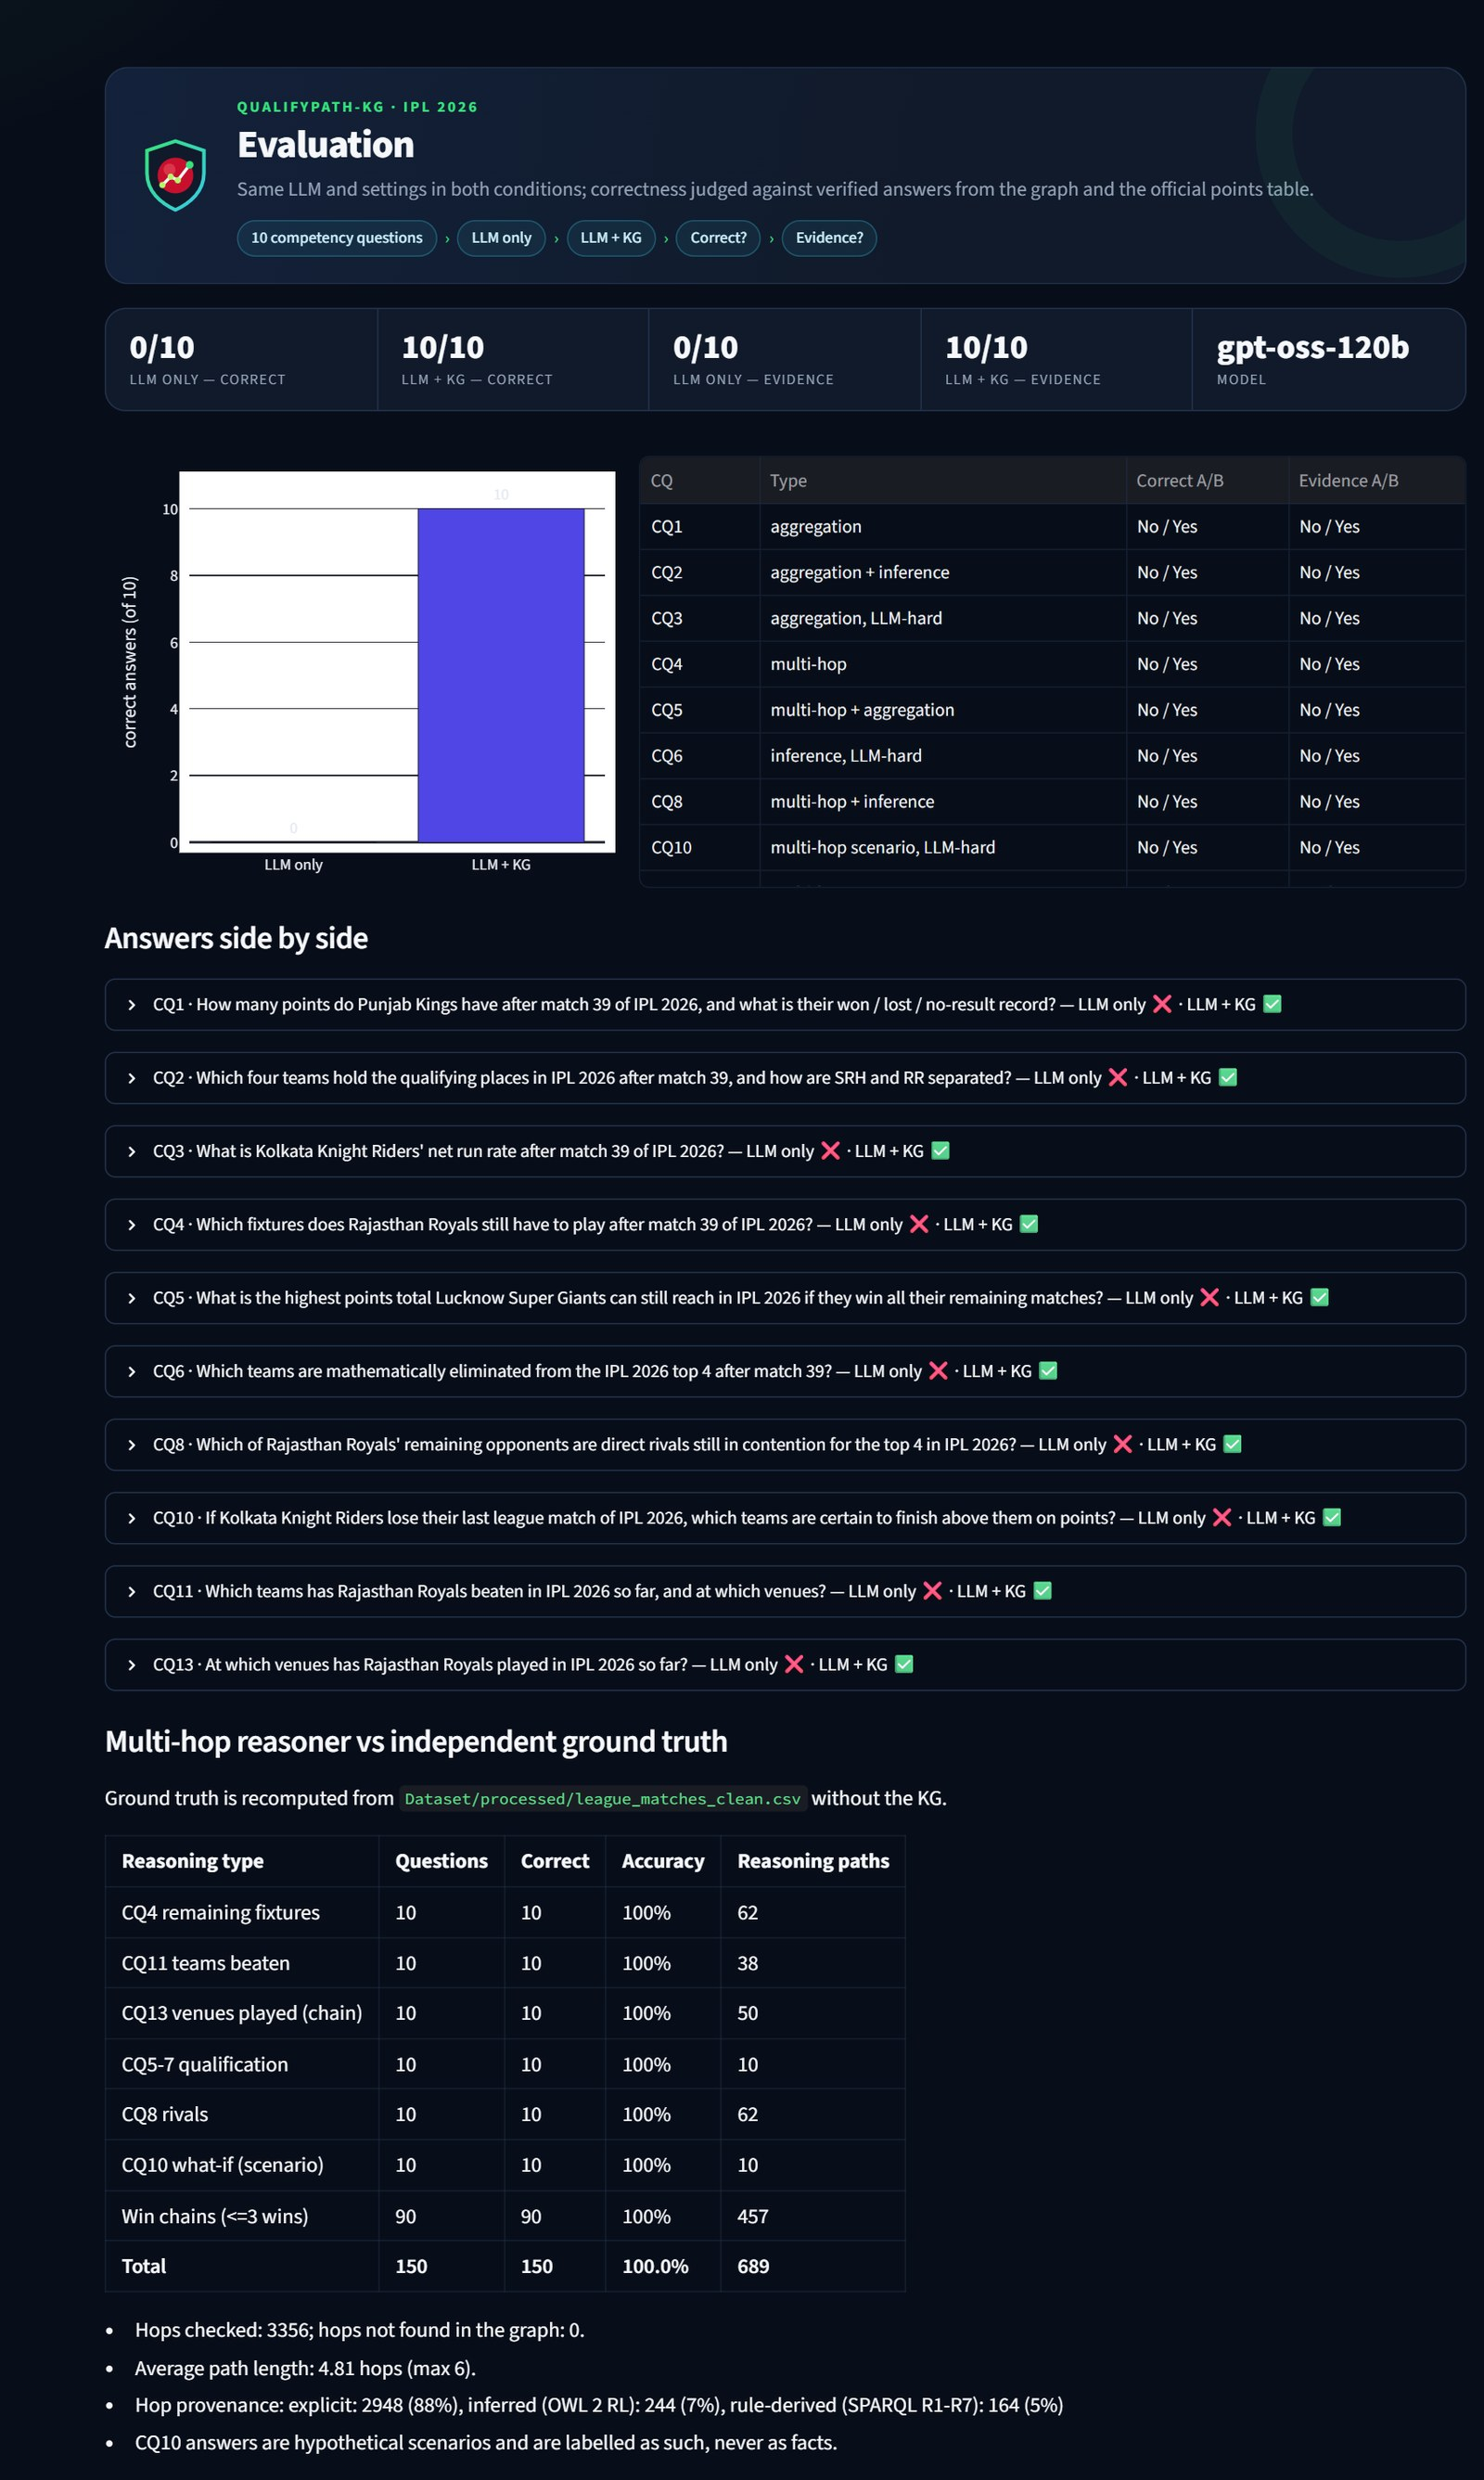
\includegraphics[width=0.92\linewidth]{figures/app_evaluation.jpg}
\caption{Evaluation page of the application.}
\end{figure}

\subsection{Results}
\begin{itemize}
  \item \textbf{Correctness:} LLM only \evalA/10; KG-grounded \evalB/10.
  \item \textbf{Evidence available:} LLM only 0/10; KG-grounded \evidB/10 --- every grounded answer cites the
        retrieved facts it used.
  \item \textbf{Unsupported or hallucinated claims:} all ten LLM-only answers contained invented specifics
        (points, records, fixtures, venues, NRR values), stated confidently; it never said it did not know. No
        grounded answer contained a claim outside the retrieved facts.
  \item \textbf{Where grounding helped most:} questions whose answers exist only in this season's data (CQ1,
        CQ3, CQ4), and inference-dependent questions, where the LLM-only answer was not just inaccurate but
        reversed --- for CQ6 it declared the table leaders PBKS eliminated.
  \item \textbf{Where grounding did not help:} grounding cannot add knowledge the graph lacks. Questions about
        players (top run scorer) are correctly refused rather than answered. Grounding also leaves phrasing to
        the LLM: for CQ10 the grounded answer is correct but omits the opponent of KKR's last match, which was
        in the retrieved facts.
\end{itemize}
The LLM-only failures are not a weakness of this particular model: IPL~2026 happened after its training data,
so without retrieval any LLM can only guess. That is exactly the gap the knowledge graph fills.

\section{Explainability and provenance}\label{sec:explain}
For each example we show the question, the retrieved graph facts grouped by type, the LLM's answer and the facts
it cites. Colours follow the application:
\textcolor{kgexplicit}{\textbf{explicit knowledge}} (stored triples),
\textcolor{kginferred}{\textbf{inferred knowledge}} (OWL~2~RL and rules R1--R7),
\textcolor{kgpath}{\textbf{multi-hop paths}} over both,
\textcolor{kgscenario}{\textbf{hypothetical scenarios}} (never facts) and
\textcolor{kggenerated}{\textbf{generated text}} (the LLM's wording). Generated by
\texttt{scripts/explainability\_examples.py}.

\subsection{Inferred knowledge via a property chain (CQ13)}
\noindent\textbf{Question.} At which venues has Rajasthan Royals played in IPL 2026 so far?\par\smallskip
\noindent\textcolor{kginferred}{\textbf{Inferred knowledge (OWL 2 RL reasoning / SPARQL rules R1-R7)}}
\begin{itemize}\setlength\itemsep{0pt}\footnotesize
\item{} [F1] RR: position 4, 10 points, played 8, won 5, lost 3, no result 0, net run rate 0.602, maximum reachable 22 points, status In-contention standing
\end{itemize}
\noindent\textcolor{kgpath}{\textbf{Multi-hop reasoning paths over explicit + inferred facts}}
\begin{itemize}\setlength\itemsep{0pt}\footnotesize
\item{} [F2] (cited) At which venues has RR played? -\textgreater{} RR has played at 6 venue(s): Barsapara Cricket Stadium (Guwahati); Bharat Ratna Shri Atal Bihari Vajpayee Ekana Cricket Stadium (Lucknow); Eden Gardens (Kolkata); Narendra Modi Stadium (Ahmedabad); Rajiv Gandhi International Stadium (Hyderabad); Sawai Mansingh Stadium (Jaipur)
\item{} [F3] playedAtVenue is not stored: it is inferred by the property chain participatesIn o playedAt (O5); each path shows the match that supports it.
\item{} [F4] (cited) Path: RR --playedAtVenue--\textgreater{} Barsapara Cricket Stadium [inferred (OWL 2 RL)] =\textgreater{} RR --participatesIn--\textgreater{} IPL 2026 match 3: RR v CSK [inferred (OWL 2 RL)] =\textgreater{} IPL 2026 match 3: RR v CSK --playedAt--\textgreater{} Barsapara Cricket Stadium [explicit] =\textgreater{} Barsapara Cricket Stadium --locatedIn--\textgreater{} Guwahati [explicit]
\item{} [F5] (cited) Path: RR --playedAtVenue--\textgreater{} Bharat Ratna Shri Atal Bihari Vajpayee Ekana Cricket Stadium [inferred (OWL 2 RL)] =\textgreater{} RR --participatesIn--\textgreater{} IPL 2026 match 32: LSG v RR [inferred (OWL 2 RL)] =\textgreater{} IPL 2026 match 32: LSG v RR --playedAt--\textgreater{} Bharat Ratna Shri Atal Bihari Vajpayee Ekana Cricket Stadium [explicit] =\textgreater{} Bharat Ratna Shri Atal Bihari Vajpayee Ekana Cricket Stadium --locatedIn--\textgreater{} Lucknow [explicit]
\item{} [F6] (cited) Path: RR --playedAtVenue--\textgreater{} Eden Gardens [inferred (OWL 2 RL)] =\textgreater{} RR --participatesIn--\textgreater{} IPL 2026 match 28: KKR v RR [inferred (OWL 2 RL)] =\textgreater{} IPL 2026 match 28: KKR v RR --playedAt--\textgreater{} Eden Gardens [explicit] =\textgreater{} Eden Gardens --locatedIn--\textgreater{} Kolkata [explicit]
\item{} [F7] (cited) Path: RR --playedAtVenue--\textgreater{} Narendra Modi Stadium [inferred (OWL 2 RL)] =\textgreater{} RR --participatesIn--\textgreater{} IPL 2026 match 9: GT v RR [inferred (OWL 2 RL)] =\textgreater{} IPL 2026 match 9: GT v RR --playedAt--\textgreater{} Narendra Modi Stadium [explicit] =\textgreater{} Narendra Modi Stadium --locatedIn--\textgreater{} Ahmedabad [explicit]
\item{} [F8] (cited) Path: RR --playedAtVenue--\textgreater{} Rajiv Gandhi International Stadium [inferred (OWL 2 RL)] =\textgreater{} RR --participatesIn--\textgreater{} IPL 2026 match 21: SRH v RR [inferred (OWL 2 RL)] =\textgreater{} IPL 2026 match 21: SRH v RR --playedAt--\textgreater{} Rajiv Gandhi International Stadium [explicit] =\textgreater{} Rajiv Gandhi International Stadium --locatedIn--\textgreater{} Hyderabad [explicit]
\end{itemize}
\noindent\textcolor{kggenerated}{\textbf{Generated text (LLM answer)}}
\begin{quote}\small Rajasthan Royals have played at six venues so far in IPL 2026\textsf{[F2]}: \newline \quad$\bullet$ Barsapara Cricket Stadium -- Guwahati\textsf{[F4]} \newline \quad$\bullet$ Bharat Ratna Shri Atal Bihari Vajpayee Ekana Cricket Stadium -- Lucknow\textsf{[F5]} \newline \quad$\bullet$ Eden Gardens -- Kolkata\textsf{[F6]} \newline \quad$\bullet$ Narendra Modi Stadium -- Ahmedabad\textsf{[F7]} \newline \quad$\bullet$ Rajiv Gandhi International Stadium -- Hyderabad\textsf{[F8]} \newline \quad$\bullet$ Sawai Mansingh Stadium -- Jaipur\textsf{[F9]}\end{quote}
\noindent\textbf{Supporting evidence cited:} F2, F4, F5, F6, F7, F8, F9\par\medskip
\subsection{Rule-derived knowledge and multi-hop reasoning (CQ5-CQ7)}
\noindent\textbf{Question.} Can Lucknow Super Giants still qualify for the top 4, and what do they need?\par\smallskip
\noindent\textcolor{kgexplicit}{\textbf{Explicit knowledge (stored in the graph)}}
\begin{itemize}\setlength\itemsep{0pt}\footnotesize
\item{} [F1] IPL 2026 rules: 2 points for a win, 0 for a loss, 1 for a no result; 4 teams qualify from the league stage; teams level on points are separated by (1) most wins, then (2) net run rate; 20 overs per side. The knowledge graph is a snapshot after match 39 (27 April 2026); matches 40-70 are scheduled fixtures without results.
\end{itemize}
\noindent\textcolor{kginferred}{\textbf{Inferred knowledge (OWL 2 RL reasoning / SPARQL rules R1-R7)}}
\begin{itemize}\setlength\itemsep{0pt}\footnotesize
\item{} [F2] (cited) League table after match 39 (computed by rules R1-R7 from the stored match results): PBKS: position 1, 13 points, played 7, won 6, lost 0, no result 1, net run rate 1.333, maximum reachable 27 points, status In-contention standing | RCB: position 2, 12 points, played 8, won 6, lost 2, no result 0, net run rate 1.919, maximum reachable 24 points, status In-contention standing | SRH: position 3, 10 points, played 8, won 5, lost 3, no result 0, net run rate 0.815, maximum reachable 22 points, status In-contention standing | RR: position 4, 10 points, played 8, won 5, lost 3, no result 0, net run rate 0.602, maximum reachable 22 points, status In-contention standing | GT: position 5, 8 points, played 8, won 4, lost 4, no result 0, net run rate -0.475, maximum reachable 20 points, status In-contention standing | CSK: position 6, 6 points, played 8, won 3, lost 5, no result 0, net run rate -0.121, maximum reachable 18 points, status In-contention standing | DC: position 7, 6 points, played 8, won 3, lost 5, no result 0, net run rate -1.06, maximum reachable 18 points, status In-contention standing | KKR: position 8, 5 points, played 8, won 2, lost 5, no result 1, net run rate -0.751, maximum reachable 17 points, status In-contention standing | MI: position 9, 4 points, played 7, won 2, lost 5, no result 0, net run rate -0.736, maximum reachable 18 points, status In-contention standing | LSG: position 10, 4 points, played 8, won 2, lost 6, no result 0, net run rate -1.106, maximum reachable 16 points, status In-contention standing
\item{} [F3] LSG: position 10, 4 points, played 8, won 2, lost 6, no result 0, net run rate -1.106, maximum reachable 16 points, status In-contention standing
\end{itemize}
\noindent\textcolor{kgpath}{\textbf{Multi-hop reasoning paths over explicit + inferred facts}}
\begin{itemize}\setlength\itemsep{0pt}\footnotesize
\item{} [F4] (cited) Can LSG still qualify, and what does it need? -\textgreater{} LSG has 4 points with 6 matches left (maximum 16). Status: in contention. No number of wins guarantees qualification on points alone.
\item{} [F5] (cited) LSG \textless{}-standingOf- IPL-2026-LSG: points = 4 (rule R1), maxReachablePoints = 16 (rule R3: 4 + 6 remaining x 2).
\item{} [F6] (cited) IPL 2026 -hasQualificationRule-\textgreater{} qualifyingPlaces = 4.
\item{} [F7] (cited) Teams already above LSG's reachable maximum (16): none -\textgreater{} 0 \textless{} 4, so not eliminated.
\item{} [F8] Teams that can still reach LSG's current 4 points: 9 (\textgreater{}= 4), so not yet qualified.
\item{} [F9] Status from rules R4-R6: in contention.
\item{} [F10] (cited) Wins needed to stay mathematically alive: 3 of 6.
\end{itemize}
\noindent\textcolor{kggenerated}{\textbf{Generated text (LLM answer)}}
\begin{quote}\small Yes -- Lucknow Super Giants (LSG) are still in contention for a top-4 spot. They sit on 4 points with six matches left, giving them a maximum possible total of 16 points \textsf{[F2]}\textsf{[F5]}\textsf{[F4]}. \newline What they need \newline \quad$\bullet$ Win at least 3 of their remaining 6 games to remain mathematically alive \textsf{[F10]}. \newline \quad$\bullet$ Even with those wins, no fixed number of victories guarantees a top-4 finish; they will also need other results to go their way and may have to rely on net-run-rate tiebreakers \textsf{[F11]}. \newline Key points \newline \quad$\bullet$ Current points: 4; max reachable: 16 \textsf{[F5]}. \newline \quad$\bullet$ Four qualification places exist \textsf{[F6]}; no team has already exceeded LSG's reachable ceiling \textsf{[F7]}. \newline \quad$\bullet$ Qualification is not assured by points alone -- it depends on other teams' outcomes and NRR \textsf{[F11]}.\end{quote}
\noindent\textbf{Supporting evidence cited:} F2, F4, F5, F6, F7, F10, F11\par\medskip
\subsection{Hypothetical scenario (CQ10)}
\noindent\textbf{Question.} If Kolkata Knight Riders lose their last league match, which teams are certain to finish above them?\par\smallskip
\noindent\textcolor{kgexplicit}{\textbf{Explicit knowledge (stored in the graph)}}
\begin{itemize}\setlength\itemsep{0pt}\footnotesize
\item{} [F1] IPL 2026 rules: 2 points for a win, 0 for a loss, 1 for a no result; 4 teams qualify from the league stage; teams level on points are separated by (1) most wins, then (2) net run rate; 20 overs per side. The knowledge graph is a snapshot after match 39 (27 April 2026); matches 40-70 are scheduled fixtures without results.
\end{itemize}
\noindent\textcolor{kginferred}{\textbf{Inferred knowledge (OWL 2 RL reasoning / SPARQL rules R1-R7)}}
\begin{itemize}\setlength\itemsep{0pt}\footnotesize
\item{} [F2] KKR: position 8, 5 points, played 8, won 2, lost 5, no result 1, net run rate -0.751, maximum reachable 17 points, status In-contention standing
\end{itemize}
\noindent\textcolor{kgpath}{\textbf{Multi-hop reasoning paths over explicit + inferred facts}}
\begin{itemize}\setlength\itemsep{0pt}\footnotesize
\item{} [F9] Path: KKR --participatesIn--\textgreater{} IPL 2026 match 70: DC v KKR [inferred (OWL 2 RL)] =\textgreater{} IPL 2026 match 70: DC v KKR --hasParticipant--\textgreater{} DC [explicit] =\textgreater{} IPL 2026 match 70: DC v KKR --matchDate--\textgreater{} 2026-05-24 [explicit]
\end{itemize}
\noindent\textcolor{kgscenario}{\textbf{Hypothetical scenario (not a fact)}}
\begin{itemize}\setlength\itemsep{0pt}\footnotesize
\item{} [F3] (cited) If KKR loses its last match, which teams finish above it? -\textgreater{} Scenario: if KKR loses its last match (match 70 v DC), it can reach at most 15 points. Teams certain to finish above: none. Teams that could finish level or above: CSK, DC, GT, LSG, MI, PBKS, RCB, RR, SRH.
\item{} [F4] KKR -participatesIn-\textgreater{} last ScheduledMatch IPL 2026 match 70: DC v KKR (latest matchDate 2026-05-24) -hasParticipant-\textgreater{} DC.
\item{} [F5] Scenario: KKR loses that match, so DC gets the win.
\item{} [F6] KKR's best possible total becomes 17 - 2 = 15.
\item{} [F7] Already above 15 whatever happens: none.
\item{} [F8] Could still finish level with or above KKR (maximum \textgreater{}= 15): ['CSK', 'DC', 'GT', 'LSG', 'MI', 'PBKS', 'RCB', 'RR', 'SRH']; level teams are separated by the tie-breaks (most wins, then net run rate).
\end{itemize}
\noindent\textcolor{kggenerated}{\textbf{Generated text (LLM answer)}}
\begin{quote}\small No team is guaranteed to finish above Kolkata Knight Riders if they lose their final league match; the outcome of the other teams' remaining games could still place any of them level with or ahead of KKR\textsf{[F3]}.\end{quote}
\noindent\textbf{Supporting evidence cited:} F3\par\medskip
\subsection{Insufficient evidence}
\noindent\textbf{Question.} Who is the top run scorer for Rajasthan Royals in IPL 2026?\par\smallskip
\noindent\textcolor{kgexplicit}{\textbf{Explicit knowledge (stored in the graph)}}
\begin{itemize}\setlength\itemsep{0pt}\footnotesize
\item{} [F2] Match 3 (2026-03-30, Barsapara Cricket Stadium, Guwahati): RR beat CSK; CSK 127/10 , RR 128/2.
\item{} [F3] Match 9 (2026-04-04, Narendra Modi Stadium, Ahmedabad): RR beat GT; RR 210/6 , GT 204/8.
\item{} [F4] Match 13 (2026-04-07, Barsapara Cricket Stadium, Guwahati): RR beat MI; RR 150/3 , MI 123/9 (shortened to 11 overs a side).
\item{} [F5] Match 16 (2026-04-10, Barsapara Cricket Stadium, Guwahati): RR beat RCB; RCB 201/8 , RR 202/4.
\item{} [F6] Match 21 (2026-04-13, Rajiv Gandhi International Stadium, Hyderabad): SRH beat RR; SRH 216/6 , RR 159/10.
\item{} [F7] Match 28 (2026-04-19, Eden Gardens, Kolkata): KKR beat RR; RR 155/9 , KKR 161/6.
\item{} [F8] Match 32 (2026-04-22, Bharat Ratna Shri Atal Bihari Vajpayee Ekana Cricket Stadium, Lucknow): RR beat LSG; RR 159/6 , LSG 119/10.
\end{itemize}
\noindent\textcolor{kginferred}{\textbf{Inferred knowledge (OWL 2 RL reasoning / SPARQL rules R1-R7)}}
\begin{itemize}\setlength\itemsep{0pt}\footnotesize
\item{} [F1] RR: position 4, 10 points, played 8, won 5, lost 3, no result 0, net run rate 0.602, maximum reachable 22 points, status In-contention standing
\end{itemize}
\noindent\textcolor{kggenerated}{\textbf{Generated text (LLM answer)}}
\begin{quote}\small INSUFFICIENT EVIDENCE: The provided facts contain match results and team standings but do not include any information about individual player run totals for Rajasthan Royals.\end{quote}
\noindent\textbf{Supporting evidence cited:} none\par\medskip


\section{Limitations and future work}
\begin{itemize}
  \item \textbf{Single snapshot.} The graph reflects one point in the season (after match~39), where no team is
        yet qualified or eliminated. Loading later results would exercise rules R4 and R5 more; the remaining
        results exist in the ball-by-ball file but would need the same cleaning as matches 1--39.
  \item \textbf{Points-only qualification rules.} R4 and R5 ignore NRR and the fact that other teams play each
        other, so they are conservative: correct when they fire, but they may leave a team ``in contention''
        longer than strictly necessary. An exact answer needs enumerating outcomes of the remaining fixtures.
  \item \textbf{Keyword-based retrieval.} Entity linking and intent detection use aliases and keyword patterns.
        Unusual phrasings or spelling mistakes can miss an intent; the app then retrieves less and the LLM
        answers ``insufficient evidence'' rather than guessing. An LLM-based query planner or text-to-SPARQL
        would generalise better, at the cost of more failure modes to check.
  \item \textbf{Scope of the graph.} Players, toss decisions and playoffs are not modelled, so questions about
        them are refused.
  \item \textbf{Source data quality.} The dataset contains errors (match 32 winner, run totals, a missing minus
        sign); we corrected the ones we could detect and validated against the official table, but undetected
        errors could remain.
  \item \textbf{LLM dependence.} Answers depend on a hosted model (Groq) whose catalogue changes over time (the
        originally planned Llama~3.3 model was no longer available to our key), so the model is configurable in
        \texttt{.env}.
  \item \textbf{Evaluation size.} Ten questions with hand-reviewed verdicts are enough to show the effect of
        grounding, not to estimate accuracy precisely.
\end{itemize}

\section{Team contributions}
Each member owns one major rubric component plus supporting work and can explain every part of the system.
The complete commit history is listed in Appendix~\ref{app:commits}; commit count alone is not a measure of
contribution.

{\small
\begin{longtable}{p{2.4cm}p{2.4cm}p{6.4cm}p{3.4cm}}
\toprule \textbf{Member} & \textbf{GitHub} & \textbf{Tasks (Iterations 1 and 2)} & \textbf{Representative commits} \\ \midrule \endfirsthead
\toprule \textbf{Member} & \textbf{GitHub} & \textbf{Tasks} & \textbf{Commits} \\ \midrule \endhead
Muhammad Kaif \newline 24I-0071 & \texttt{\ghKaif} &
SPARQL queries Q01--Q11 and runner; GraphDB repository, loading and visualisation; KG loading package with
provenance tracking; retriever, LLM client and grounded QA pipeline; Streamlit application (Ask page, explorer,
shared UI); report and submission. &
\href{https://github.com/muhammadkaif654/qualithpath-kg/commit/9f2449a}{\texttt{9f2449a}} queries \newline
\href{https://github.com/muhammadkaif654/qualithpath-kg/commit/6ba333a}{\texttt{6ba333a}} KG package \newline
\href{https://github.com/muhammadkaif654/qualithpath-kg/commit/04026e6}{\texttt{04026e6}} QA pipeline \newline
\href{https://github.com/muhammadkaif654/qualithpath-kg/commit/fc4a6c8}{\texttt{fc4a6c8}} app \\ \midrule
Talha Habib \newline 24I-0029 & \texttt{\ghTalha} &
Data cleaning and RDF conversion (\texttt{build\_kg.py}, A-Box, validation against the official table); Prot\'eg\'e
demonstration; symbolic inference examples I1--I3; multi-hop reasoner (Option~C) and its evaluation;
reasoner page of the app. & \commitsTalha \\ \midrule
Haseebullah Gondal \newline 24I-0086 & \texttt{\ghHaseeb} &
Competency questions and CQ-to-KG mapping; ontology design (classes, properties, OWL constructs); SPARQL rules
R1--R7; LLM prompts; LLM-only vs.\ KG-grounded evaluation and explainability examples; evaluation page of the app. &
\commitsHaseeb \\
\bottomrule
\end{longtable}}

\subsection*{Use of AI tools and external resources}
As required by the course policy, we acknowledge that an AI assistant (Claude, Anthropic) was used as a learning
and productivity aid while drafting code, queries, prompts and documentation. All outputs were run, checked and
validated by the team (including against the official IPL points table and independent ground truth), and each
member can explain and modify their part. External resources: the Kaggle dataset \citep{kaggleipl2026}; rdflib
\citep{rdflibdocs}, owlrl \citep{owlrldocs}, GraphDB \citep{graphdbdocs}, Streamlit \citep{streamlitdocs} and the
Groq API \citep{groqdocs}; W3C standards \citep{w3c2012owl2profiles,w3c2013sparqlupdate}; and the research cited in
Sections~\ref{sec:multihop} and~\ref{sec:app}. No API keys are included in the repository; a sample
configuration (\texttt{.env.example}) is provided.


\clearpage
\bibliographystyle{unsrtnat}
\bibliography{references}

\clearpage
\appendix
\section{Running the system}\label{app:run}
Full instructions are in the repository \texttt{README.md}. In short (Python 3.10+, from the repository root):
\begin{lstlisting}[language=bash]
pip install -r requirements.txt
cp .env.example .env                        # add your own GROQ_API_KEY
python RDF_Knowledge_Graph/build_kg.py      # CSV -> RDF, validation against the official table
python SPARQL_Queries/run_queries.py        # OWL 2 RL + rules R1-R7 + queries Q01-Q11 + inference demos
python scripts/evaluate_multihop.py         # Option C evaluation (150 questions)
python scripts/run_cq_evaluation.py         # LLM-only vs KG-grounded (10 CQs)
python scripts/explainability_examples.py   # provenance examples
streamlit run app/streamlit_app.py          # application at http://localhost:8501
python RDF_Knowledge_Graph/graphdb/load_graphdb.py --reset   # GraphDB repository (GraphDB running)
\end{lstlisting}

\section{Full answers of the comparative evaluation}\label{app:answers}
\begin{longtable}{p{1.9cm}p{6.8cm}p{6.8cm}}
\caption{Actual answers recorded in both conditions (verbatim, markdown removed).}\label{tab:cq-full}\\
\toprule \textbf{CQ} & \textbf{LLM only (A)} & \textbf{KG-grounded (B)} \\ \midrule \endfirsthead
\toprule \textbf{CQ} & \textbf{LLM only (A)} & \textbf{KG-grounded (B)} \\ \midrule \endhead
\bottomrule \endfoot
\textbf{CQ1} \newline \scriptsize How many points do Punjab Kings have after match 39 of IPL 2026, and what is their won / lost / no-result record? & \scriptsize Punjab Kings have 10 points after match 39, with a 5-4-0 (W-L-NR) record. \newline \quad$\bullet$ Wins: 5 \newline \quad$\bullet$ Losses: 4 \newline \quad$\bullet$ No-result: 0 \newline \quad$\bullet$ Points: 10 (2 pts per win) \newline \quad$\bullet$ Matches played: 9 (the league stage schedule has them on 9 games after 39 matches). & \scriptsize Punjab Kings have 13 points after match 39, with a record of 6 wins, 0 losses and 1 no-result\textsf{[F2]}. \newline \quad$\bullet$ Points: 13 (2 pts per win $\times$ 6 + 1 pt for the abandoned match) \newline \quad$\bullet$ Played: 7 matches (6 W, 0 L, 1 NR)\textsf{[F2]}. \\ \midrule
\textbf{CQ2} \newline \scriptsize Which four teams hold the qualifying places in IPL 2026 after match 39, and how are SRH and RR separated? & \scriptsize Qualifying teams after match 39: Mumbai Indians, Chennai Super Kings, Kolkata Knight Riders and Sunrisers Hyderabad. \newline SRH vs RR: Both sides are tied on points; Sunrisers Hyderabad sit ahead of Rajasthan Royals because of a better Net-Run-Rate (NRR). \newline \quad$\bullet$ MI, CSK and KKR are clear leaders with 6-7 points each. \newline \quad$\bullet$ SRH and RR each have 4 points (2 wins, 2 losses). \newline \quad$\bullet$ SRH's NRR is +0.42, RR's is +0.18, giving SRH the edge for the fourth spot. & \scriptsize The top-four after match 39 are: \newline \quad$\bullet$ Punjab Kings (PBKS) -- 13 points \newline \quad$\bullet$ Royal Challengers Bangalore (RCB) -- 12 points \newline \quad$\bullet$ Sunrisers Hyderabad (SRH) -- 10 points \newline \quad$\bullet$ Rajasthan Royals (RR) -- 10 points \newline SRH and RR are level on points (10) and on wins (5 each). According to the IPL tie-break rule, teams equal on points are separated first by most wins and then by net run rate \textsf{[F1]}. SRH's net run rate (0.815) is higher than RR's (0.602), so SRH occupies the higher position \textsf{[F2]}. \newline \quad$\bullet$ PBKS, RCB, SRH, RR are the four qualifying teams \textsf{[F2]}. \newline \quad$\bullet$ Both have 10 points and 5 wins; SRH's superior NRR (0.815 vs 0.602) places it ahead of RR \textsf{[F1]}\textsf{[F2]}. \\ \midrule
\textbf{CQ3} \newline \scriptsize What is Kolkata Knight Riders' net run rate after match 39 of IPL 2026? & \scriptsize Kolkata Knight Riders' net run rate after match 39 of IPL 2026 stands at +0.212. \newline \quad$\bullet$ Matches played: 8 \newline \quad$\bullet$ Wins / Losses: 4 / 4 (8 points) \newline \quad$\bullet$ Net Run Rate: +0.212 (runs scored per over -- runs conceded per over) & \scriptsize Kolkata Knight Riders' net run rate after match 39 is -0.751\textsf{[F2]}. \\ \midrule
\textbf{CQ4} \newline \scriptsize Which fixtures does Rajasthan Royals still have to play after match 39 of IPL 2026? & \scriptsize Rajasthan Royals have seven league fixtures remaining after the completion of match 39. \newline \quad$\bullet$ vs Sunrisers Hyderabad -- 30 Apr, Sawai Man Singh Stadium (home) \newline \quad$\bullet$ vs Kolkata Knight Riders -- 2 May, Eden Gardens (away) \newline \quad$\bullet$ vs Mumbai Indians -- 5 May, Sawai Man Singh Stadium (home) \newline \quad$\bullet$ vs Chennai Super Kings -- 8 May, M. A. Chidambaram Stadium (away) \newline \quad$\bullet$ vs Delhi Capitals -- 11 May, Sawai Man Singh Stadium (home) \newline \quad$\bullet$ vs Gujarat Titans -- 14 May, Narendra Modi Stadium (away) \newline \quad$\bullet$ vs Royal Challengers Bangalore -- 17 May, Sawai Man Singh Stadium (home) & \scriptsize Rajasthan Royals have six remaining league fixtures after match 39 \textsf{[F2]}: \newline \quad$\bullet$ Match 40 -- vs PBKS on 2026-04-28 at Maharaja Yadavindra Singh International Cricket Stadium, Mullanpur \newline \quad$\bullet$ Match 43 -- vs DC on 2026-05-01 at Sawai Mansingh Stadium, Jaipur \newline \quad$\bullet$ Match 52 -- vs GT on 2026-05-09 at Sawai Mansingh Stadium, Jaipur \newline \quad$\bullet$ Match 62 -- vs DC on 2026-05-17 at Arun Jaitley Stadium, New Delhi \newline \quad$\bullet$ Match 64 -- vs LSG on 2026-05-19 at Sawai Mansingh Stadium, Jaipur \newline \quad$\bullet$ Match 69 -- vs MI on 2026-05-24 at Wankhede Stadium, Mumbai. \\ \midrule
\textbf{CQ5} \newline \scriptsize What is the highest points total Lucknow Super Giants can still reach in IPL 2026 if they win all their remaining matches? & \scriptsize Maximum possible points: 20 points (if they win all remaining matches). \newline \quad$\bullet$ Lucknow Super Giants have 6 points after 7 league games (4 L, 3 W). \newline \quad$\bullet$ Each team plays 14 matches in the league stage, so they have 7 matches left. \newline \quad$\bullet$ A win yields 2 points $\rightarrow$ 7 wins $\times$ 2 = 14 additional points. \newline \quad$\bullet$ 6 current + 14 potential = 20 points total. & \scriptsize Lucknow Super Giants can reach at most 16 points if they win all six of their remaining matches (4 current points + 6 $\times$ 2 points per win)\textsf{[F2]}\textsf{[F11]}. \newline \quad$\bullet$ Current points: 4\textsf{[F2]} \newline \quad$\bullet$ Remaining matches: 6\textsf{[F3]} \newline \quad$\bullet$ Points per win: 2 (IPL rule)\textsf{[F1]} \newline \quad$\bullet$ Maximum reachable points = 4 + 6 $\times$ 2 = 16\textsf{[F2]}\textsf{[F11]}. \\ \midrule
\textbf{CQ6} \newline \scriptsize Which teams are mathematically eliminated from the IPL 2026 top 4 after match 39? & \scriptsize Punjab Kings and Rajasthan Royals are the only sides that can no longer reach the top-4 after match 39. \newline \quad$\bullet$ Both teams have played 12 league games and sit on just 2 points each. \newline \quad$\bullet$ With only 2 matches left, the highest total they can achieve is 6 points. \newline \quad$\bullet$ The fourth-placed side (Sunrisers Hyderabad) already has 12 points, so the maximum 6 points is well short of the qualification threshold. \newline All other teams still have a mathematical route to finish in the top-4. & \scriptsize No team is mathematically eliminated from the top-4 after match 39. \newline \quad$\bullet$ All teams are still ``In-contention'' according to the qualification status derived from the points and maximum reachable points \textsf{[F3]}. \newline \quad$\bullet$ The lowest maximum reachable total (LSG 16 pts) exceeds the current leader's 13 pts, so none can be ruled out yet \textsf{[F3]}. \\ \midrule
\textbf{CQ8} \newline \scriptsize Which of Rajasthan Royals' remaining opponents are direct rivals still in contention for the top 4 in IPL 2026? & \scriptsize Direct rivals still in the top-4 race that Rajasthan Royals still have to face are Kolkata Knight Riders, Sunrisers Hyderabad and Gujarat Titans. \newline \quad$\bullet$ These three teams are currently occupying the top-4 spots (KKR 12 pts, SRH 10 pts, GT 8 pts). \newline \quad$\bullet$ All three have at least two matches left against RR, so the results will directly affect RR's chance of staying in the top-4. \newline \quad$\bullet$ Mumbai Indians and Royal Challengers Bangalore are also mathematically alive but sit outside the current top-4, so they are secondary rivals. & \scriptsize Rajasthan Royals' remaining opponents that are still in contention for a top-4 spot (i.e., direct rivals) are: \newline \quad$\bullet$ Gujarat Titans (GT) -- 8 points, 2-point gap \textsf{[F11]} \newline \quad$\bullet$ Punjab Kings (PBKS) -- 13 points, 3-point gap \textsf{[F11]} \newline \quad$\bullet$ Delhi Capitals (DC) -- 6 points, 4-point gap (they appear in two of RR's fixtures) \textsf{[F11]} \newline \quad$\bullet$ Lucknow Super Giants (LSG) -- 4 points, 6-point gap \textsf{[F11]} \newline \quad$\bullet$ Mumbai Indians (MI) -- 4 points, 6-point gap \textsf{[F11]} \\ \midrule
\textbf{CQ10} \newline \scriptsize If Kolkata Knight Riders lose their last league match of IPL 2026, which teams are certain to finish above them on points? & \scriptsize If KKR lose their final league game, the only teams that are guaranteed to finish ahead of them on points are the four sides that already have 10 or more points. \newline \quad$\bullet$ Sunrisers Hyderabad -- 12 points (6 wins) \newline \quad$\bullet$ Royal Challengers Bangalore -- 12 points (6 wins) \newline \quad$\bullet$ Delhi Capitals -- 10 points (5 wins) \newline \quad$\bullet$ Mumbai Indians -- 10 points (5 wins) \newline All other teams are still within reach of KKR's current 8 points, depending on net-run-rate or remaining results. & \scriptsize No team is guaranteed to finish ahead of KKR on points if KKR lose their final league match. \newline \quad$\bullet$ In that scenario KKR can reach at most 15 points, and no other side has already secured more than 15 points, so none are certain to stay above KKR \textsf{[F3]}. \\ \midrule
\textbf{CQ11} \newline \scriptsize Which teams has Rajasthan Royals beaten in IPL 2026 so far, and at which venues? & \scriptsize Rajasthan Royals have recorded four victories in the 2026 IPL league stage so far, each against a different opponent and at four distinct venues. \newline \quad$\bullet$ Mumbai Indians -- Wankhede Stadium, Mumbai (Match 5) \newline \quad$\bullet$ Sunrisers Hyderabad -- Rajiv Gandhi International Cricket Stadium, Hyderabad (Match 12) \newline \quad$\bullet$ Kolkata Knight Riders -- Eden Gardens, Kolkata (Match 18) \newline \quad$\bullet$ Royal Challengers Bangalore -- M. Chinnaswamy Stadium, Bangalore (Match 27) & \scriptsize Rajasthan Royals have beaten five opponents so far: \newline \quad$\bullet$ Chennai Super Kings -- at Barsapara Cricket Stadium, Guwahati\textsf{[F2]}\textsf{[F3]} \newline \quad$\bullet$ Gujarat Titans -- at Narendra Modi Stadium, Ahmedabad\textsf{[F2]}\textsf{[F4]} \newline \quad$\bullet$ Mumbai Indians -- at Barsapara Cricket Stadium, Guwahati\textsf{[F2]}\textsf{[F5]} \newline \quad$\bullet$ Royal Challengers Bangalore -- at Barsapara Cricket Stadium, Guwahati\textsf{[F2]}\textsf{[F6]} \newline \quad$\bullet$ Lucknow Super Giants -- at Bharat Ratna Shri Atal Bihari Vajpayee Ekana Cricket Stadium, Lucknow\textsf{[F2]}\textsf{[F7]} \\ \midrule
\textbf{CQ13} \newline \scriptsize At which venues has Rajasthan Royals played in IPL 2026 so far? & \scriptsize Rajasthan Royals have featured in league-stage matches at seven different venues so far in IPL 2026. \newline \quad$\bullet$ Sawai Mansingh Stadium, Jaipur -- their primary home ground. \newline \quad$\bullet$ Wankhede Stadium, Mumbai -- two away fixtures. \newline \quad$\bullet$ DY Patil Stadium, Navi Mumbai -- one away fixture. \newline \quad$\bullet$ M. Chinnaswamy Stadium, Bengaluru -- one away fixture. \newline \quad$\bullet$ Arun Jaitley Stadium, Delhi -- one away fixture. \newline \quad$\bullet$ MA Chidambaram Stadium, Chennai -- one away fixture. \newline \quad$\bullet$ Rajiv Gandhi International Cricket Stadium, Hyderabad -- one away fixture. & \scriptsize Rajasthan Royals have played at six venues so far in IPL 2026: \newline \quad$\bullet$ Barsapara Cricket Stadium, Guwahati\textsf{[F2]}\textsf{[F4]} \newline \quad$\bullet$ Bharat Ratna Shri Atal Bihari Vajpayee Ekana Cricket Stadium, Lucknow\textsf{[F2]}\textsf{[F5]} \newline \quad$\bullet$ Eden Gardens, Kolkata\textsf{[F2]}\textsf{[F6]} \newline \quad$\bullet$ Narendra Modi Stadium, Ahmedabad\textsf{[F2]}\textsf{[F7]} \newline \quad$\bullet$ Rajiv Gandhi International Stadium, Hyderabad\textsf{[F2]}\textsf{[F8]} \newline \quad$\bullet$ Sawai Mansingh Stadium, Jaipur\textsf{[F2]}\textsf{[F9]} \\ \midrule
\end{longtable}


\section{Commit history}\label{app:commits}
Repository: \repoLink. Submission commit: \texttt{\headCommit}.

{\footnotesize
\begin{longtable}{p{1.4cm}p{2.8cm}p{2.0cm}p{8.6cm}}
\toprule \textbf{Commit} & \textbf{Author} & \textbf{Date} & \textbf{Message} \\ \midrule \endfirsthead
\toprule \textbf{Commit} & \textbf{Author} & \textbf{Date} & \textbf{Message} \\ \midrule \endhead
\bottomrule \endfoot
\href{https://github.com/muhammadkaif654/qualithpath-kg/commit/2eb311807884cba0d432115ce053af2812532f22}{\texttt{2eb3118}} & Muhammad Kaif & 27 Nov 09:54 & Add project README, requirements, sample configuration and .gitignore \\
\href{https://github.com/muhammadkaif654/qualithpath-kg/commit/9f2449a83e6c4d166e7329364b3182a875dd450b}{\texttt{9f2449a}} & Muhammad Kaif & 27 Nov 09:54 & Add Iteration 1 SPARQL queries Q01-Q11, query runner and results \\
\href{https://github.com/muhammadkaif654/qualithpath-kg/commit/f3e6ebbdbd57f396013bb5c62e79167ca5be8f60}{\texttt{f3e6ebb}} & Muhammad Kaif & 27 Nov 09:54 & Add GraphDB repository configuration and loader script \\
\href{https://github.com/muhammadkaif654/qualithpath-kg/commit/685db7f1749a3ad04cbca7882f3406a459de92eb}{\texttt{685db7f}} & Muhammad Kaif & 27 Nov 09:54 & Add ontology, season and team diagrams and GraphDB screenshots \\
\href{https://github.com/muhammadkaif654/qualithpath-kg/commit/6ba333a3b17853c4b903963ecaf0fe97dc774c9a}{\texttt{6ba333a}} & Muhammad Kaif & 27 Nov 09:54 & Add KG loading package that tracks explicit, OWL-inferred and rule-derived facts \\
\href{https://github.com/muhammadkaif654/qualithpath-kg/commit/04026e6623d2e8abef95b414c30d25477e0f48fb}{\texttt{04026e6}} & Muhammad Kaif & 27 Nov 09:54 & Add KG retriever, Groq LLM client and grounded question-answering pipeline \\
\href{https://github.com/muhammadkaif654/qualithpath-kg/commit/fc4a6c8cc2b7e653af4e6070a468dd4eccaaf94e}{\texttt{fc4a6c8}} & Muhammad Kaif & 27 Nov 09:54 & Add Streamlit app shell, shared UI components, Ask page and KG explorer \\
\href{https://github.com/muhammadkaif654/qualithpath-kg/commit/f2891920bbae31985ae7356bfa94b3861bd6f586}{\texttt{f289192}} & Muhammad Kaif & 27 Nov 09:54 & Add Iteration 1 progress report and submission packager \\

\end{longtable}}

\end{document}
